\documentclass[8pt,xcolor=table]{beamer}

\usepackage{graphicx}
\usepackage{caption}
\usepackage{subcaption}
\usepackage{transparent}
\usepackage{epstopdf} %converting to PDF
\usepackage{multicol} 
\usepackage{animate}[2017/05/18]

% \usepackage{pdfx}
 
% \usepackage[utf8]{inputenc}
% \usepackage[T1]{fontenc}
\usepackage[table]{xcolor}    % loads also »colortbl« 
%  \usepackage{enumitem}
% \usepackage{ucltemplate}
\usepackage{color}

\usepackage{comment}

\usepackage{tabularx} % make width of table columns evenly distributed (see http://tex.stackexchange.com/questions/60601/evenly-distributing-column-widths)
% \newcolumntype{Y}{>{\centering\arraybackslash}X}

% make entire row bold or italic in table
\newcommand\setrow[1]{\gdef\rowmac{#1}#1\ignorespaces}
\newcommand\clearrow{\global\let\rowmac\relax}
\clearrow


\usepackage{amssymb}% http://ctan.org/pkg/amssymb
\usepackage{pifont}% http://ctan.org/pkg/pifont
\newcommand{\cmark}{\ding{51}}%
\newcommand{\xmark}{\ding{55}}%


%\usepackage{pgfgantt} % for grantt charts
\usepackage{rotating}
\usepackage[graphicx]{realboxes}
\usepackage[export]{adjustbox}
\usepackage{array}

\usepackage{rotating}
% \usepackage{tabularx, booktabs} % make width of table columns evenly distributed (see http://tex.stackexchange.com/questions/60601/evenly-distributing-column-widths)
% \newcolumntype{Y}{>{\centering\arraybackslash}X}

\DeclareMathOperator*{\argmin}{arg\,min}
\DeclareMathOperator*{\argmax}{arg\,max}

\usepackage{tikz}
\usetikzlibrary{arrows,positioning, shapes.symbols,shapes.callouts,patterns,shapes,chains,calc,backgrounds,fadings}

% \definecolor{parCol}{rgb}{0.1, 0.1, 1}
% \definecolor{stCol}{rgb}{0.1, 0.6, 0.1}
% \definecolor{bothCol}{rgb}{0, 0.5, 0.5}

\definecolor{parCol}{rgb}{0, 0, 0}
\definecolor{stCol}{rgb}{0, 0, 0}
\definecolor{bothCol}{rgb}{0, 0, 0}
\definecolor{blue3}{HTML}{86B7FC} % med blue
\definecolor{blue1}{HTML}{B5F1FF} % light blue
\definecolor{blue2}{HTML}{E0F9FF} % very light blue

\newcolumntype{C}[1]{>{\centering\let\newline\\\arraybackslash\hspace{0pt}}m{#1}}

\setlength{\tabcolsep}{0.2em}

 
 %% OVERVIEW OF WORK SO FAR %%
 
%Information to be included in the title page:
\title{Modelling the Neuroanatomical Progression of Alzheimer's Disease and Posterior Cortical Atrophy}
\author[Raz]{
R\u{a}zvan V. Marinescu\vspace{1em} \newline \and \small{Supervisors: Polina Golland (current), Daniel C. Alexander (previous)}}

\institute{\small{Medical Vision Group, Massachusetts Institute of Technology}

\vspace{0em}
\small{Centre for Medical Image Computing, University College London, UK}
}

\date{}

% logo of my university
\titlegraphic{
   \begin{figure}
   \begin{subfigure}{0.32\textwidth}
   \hspace{2em}
   
\includegraphics[height=1.0cm]{ucl_logo}
   \end{subfigure}
   \begin{subfigure}{0.32\textwidth}
   \centering
   
\includegraphics[height=1.0cm]{MIT_logo.png} 
   \end{subfigure}
   \begin{subfigure}{0.32\textwidth}
   \centering
   
\includegraphics[height=1.0cm]{pondLogo.png} 
   \end{subfigure}
   \end{figure}
   
   \tiny{Slides available online: https://people.csail.mit.edu/razvan/talk/martinos2019/pres.pdf}
}

\setbeamercolor{frametitle}{fg=black}
\setbeamercolor{author in head/foot}{fg=black, bg=white} 
\setbeamercolor{institute in head/foot}{fg=black, bg=white} 
\setbeamercolor{title in head/foot}{fg=black, bg=white}
\setbeamercolor{date in head/foot}{fg=black, bg=white}

\setbeamersize{text margin left=10pt,text margin right=10pt}
% \setbeamertemplate{frametitle}{
%     \vspace{0.9em}
%     \insertframetitle
% %     \vspace{-3em}
% }
\setbeamertemplate{frametitle}{%
    \vspace{0.5em}
    \usebeamerfont{frametitle}\insertframetitle%
    \vphantom{g}% To avoid fluctuations per frame
    %\hrule% Uncomment to see desired effect, without a full-width hrule
    \par% <-- added
    \hspace*{-\dimexpr0.5\paperwidth-0.5\textwidth}% <-- calculation of left margin width
    \rule[0.5\baselineskip]{\paperwidth}{0.4pt}%
}

\setbeamertemplate{footline}
{
  \vspace{-3em}
  \leavevmode%
   \rule{\paperwidth}{0.3pt}
  \hbox{%
  \begin{beamercolorbox}[wd=.2\paperwidth,ht=2.25ex,dp=1ex,center]{author in head/foot}%
    \usebeamerfont{author in head/foot}Razvan V. Marinescu
  \end{beamercolorbox}%
  \begin{beamercolorbox}[wd=.2\paperwidth,ht=2.25ex,dp=1ex,center]{institute in head/foot}%
    \usebeamerfont{institute in head/foot}razvan@csail.mit.edu
  \end{beamercolorbox}%
  \begin{beamercolorbox}[wd=.3\paperwidth,ht=2.25ex,dp=1ex,center]{institute in head/foot}%
    \usebeamerfont{institute in head/foot}https://people.csail.mit.edu/razvan/
  \end{beamercolorbox}%
  \begin{beamercolorbox}[wd=.2\paperwidth,ht=2.25ex,dp=1ex,center]{title in head/foot}%
    \usebeamerfont{title in head/foot}\insertsection
  \end{beamercolorbox}%
  \begin{beamercolorbox}[wd=.10\paperwidth,ht=2.25ex,dp=1ex,right]{date in head/foot}%
    \usebeamerfont{date in head/foot}\insertshortdate{}\hspace*{2em}
    \insertframenumber{} / \inserttotalframenumber\hspace*{2ex}
  \end{beamercolorbox}}%
  \vskip0pt%
}

% \usepackage{beamerthemesplit}

\newcommand{\backupbegin}{
   \newcounter{finalframe}
   \setcounter{finalframe}{\value{framenumber}}
}
\newcommand{\backupend}{
   \setcounter{framenumber}{\value{finalframe}}
}


\makeatletter
\long\def\beamer@author[#1]#2{%
  \def\and{\tabularnewline}
  \def\insertauthor{\def\inst{\beamer@insttitle}\def\and{\tabularnewline}%
  \begin{tabular}{rl}#2\end{tabular}}%
  \def\beamer@shortauthor{#1}%
  \ifbeamer@autopdfinfo%
    \def\beamer@andstripped{}%
    \beamer@stripands#1 \and\relax
    {\let\inst=\@gobble\let\thanks=\@gobble\def\and{, }\hypersetup{pdfauthor={\beamer@andstripped}}}
  \fi%
}
\makeatother
\beamertemplatenavigationsymbolsempty
\setbeamertemplate{caption}[numbered]
\setbeamercolor{caption name}{fg=black}
\setbeamercolor{itemize item}{fg=black}
\setbeamercolor{itemize subitem}{fg=black}
\setbeamercolor{enumerate item}{fg=black}
\setbeamercolor{enumerate subitem}{fg=black}
\setbeamertemplate{enumerate item}[default]
\setbeamertemplate{enumerate subitem}[default]

\makeatletter
\let\@@magyar@captionfix\relax
\makeatother
\begin{document}
 
\section{Introduction}

\frame{\titlepage}
 
\setbeamerfont{frametitle}{size=\large}

\newcommand{\upgradeReportLoc}{../../upgrade_report}
\newcommand{\epsrcPresLoc}{\upgradeReportLoc/epsrcPres}
\newcommand{\jointModellingDiseaseLoc}{../../jointModellingDisease}
\newcommand{\pcaLongPaperLoc}{../../PCA_long_paper}
\newcommand{\voxFld}{../../voxelwiseDPM}
\newcommand{\tadpoleFld}{../../tadpole}
\newcommand{\diffEqModelFld}{../../diffEqModel}



\newcommand*{\pcaLongFigs}{\pcaLongPaperLoc/figures}


% \includeonlyframes{1-20}
%\includeonlyframes{current}



\newcommand{\ovHeight}{2cm}


% % TODO continue with overview, move into commands
\newcommand{\ovEBM}{
\begin{subfigure}{0.47\textwidth}
\centering
1. Modelled progression of PCA and tAD\\
(using existing methods)
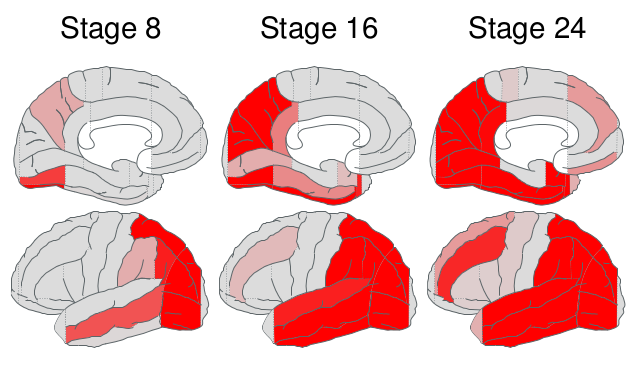
\includegraphics[height=\ovHeight]{ebm_thumb.png}
\end{subfigure}
}

\newcommand{\ovVWDPM}{
\begin{subfigure}{0.47\textwidth}
\centering
% \vspace{2.8em}
2. Developed Novel Spatio-temporal Model \\ (DIVE)\\
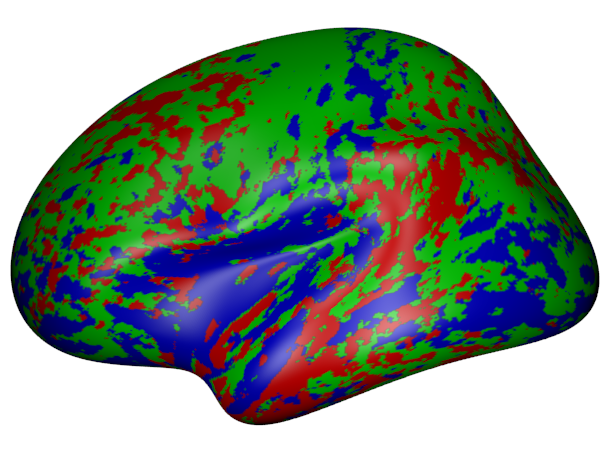
\includegraphics[height=\ovHeight]{\upgradeReportLoc/images/vwdpm/blend14_adniThavgFWHM0InithistCl3Pr0Ra1_VWDPMStd.png}
\end{subfigure}
}


\newcommand{\ovDKT}{
\begin{subfigure}{0.47\textwidth}
\centering
\vspace{2em}
3. Developed Novel Transfer Learning \\ method (DKT) \\
\vspace{0.5em}
\includegraphics[height=2.2cm]{\jointModellingDiseaseLoc/paper/figures/disease_knowledge_transfer.pdf}
\end{subfigure}
}


\newcommand{\ovTadpole}{
\begin{subfigure}{0.47\textwidth}
\centering
\vspace{-2em}
4. Organised TADPOLE Competition\\
\vspace{1em}
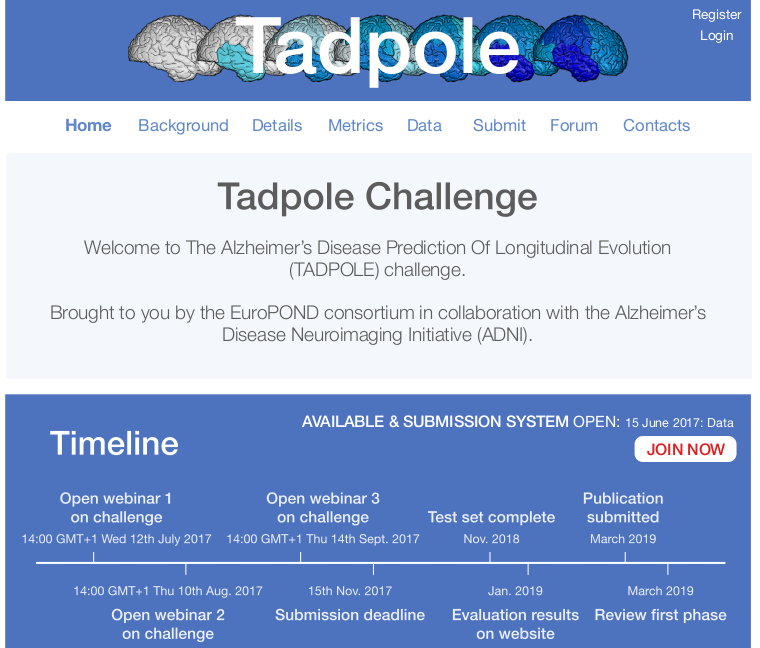
\includegraphics[height=1.2cm,valign=t]{\upgradeReportLoc/epsrcPres/tadpole} 
\end{subfigure}
}

\newcommand{\ovPainter}{
\begin{subfigure}{\textwidth}
\centering
\vspace{0.5em}
5. Created BrainPainter software\\
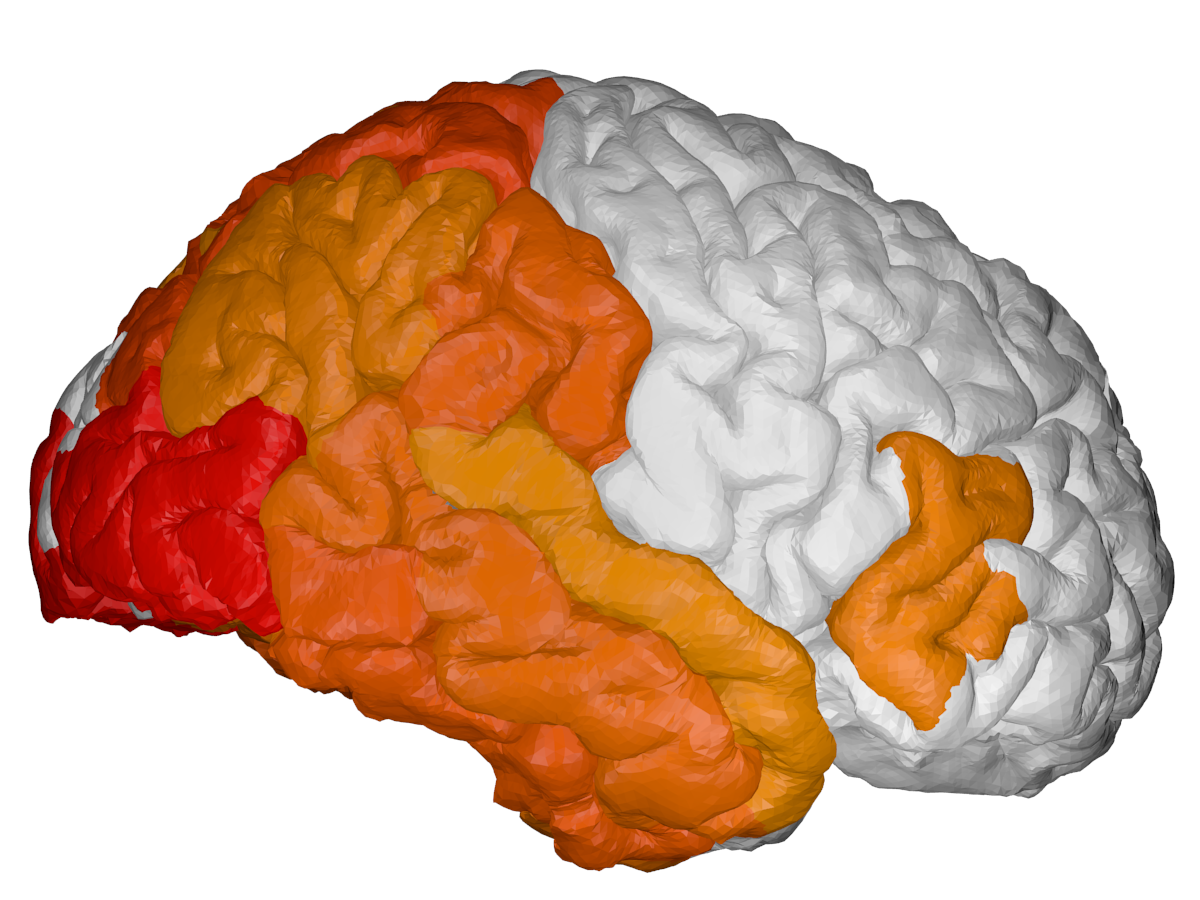
\includegraphics[height=1.5cm]{cortical-front_1}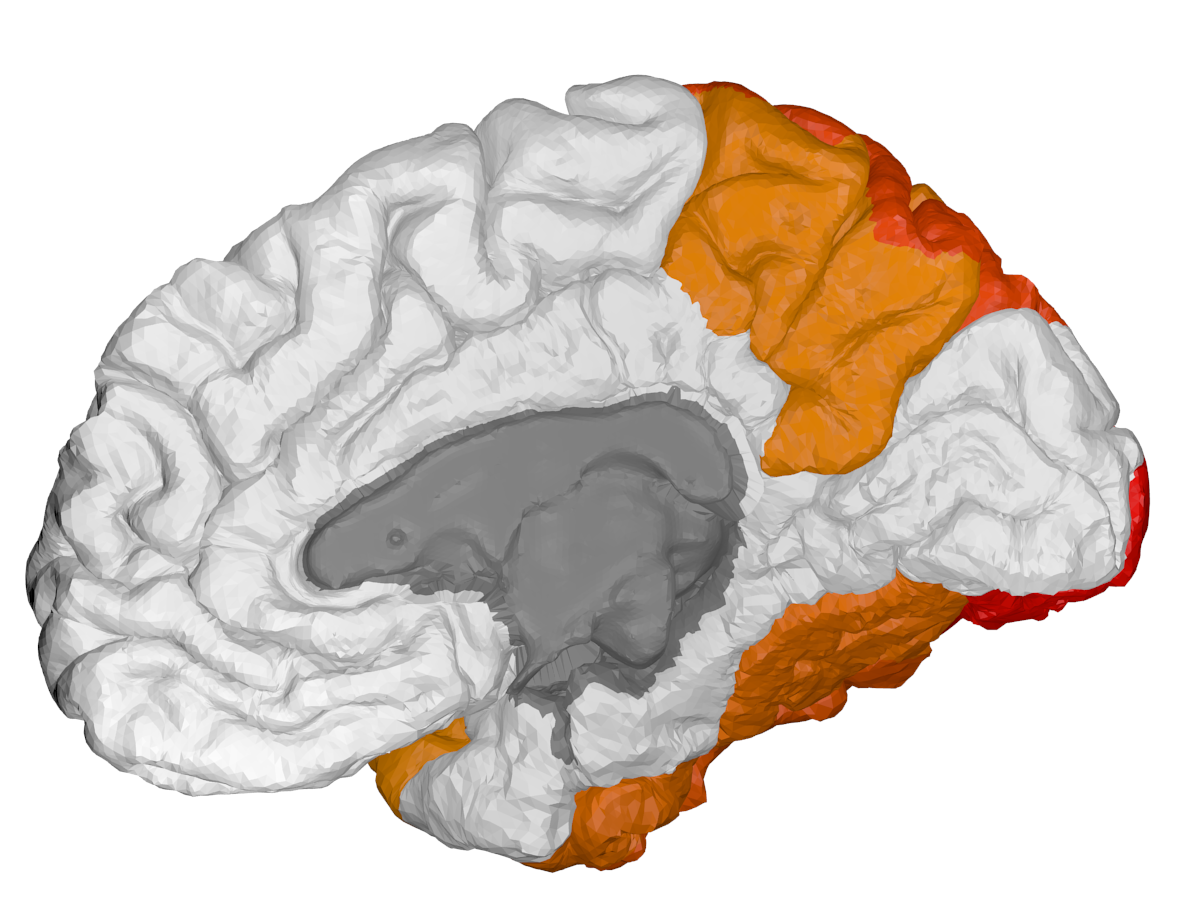
\includegraphics[height=1.5cm]{cortical-back_1}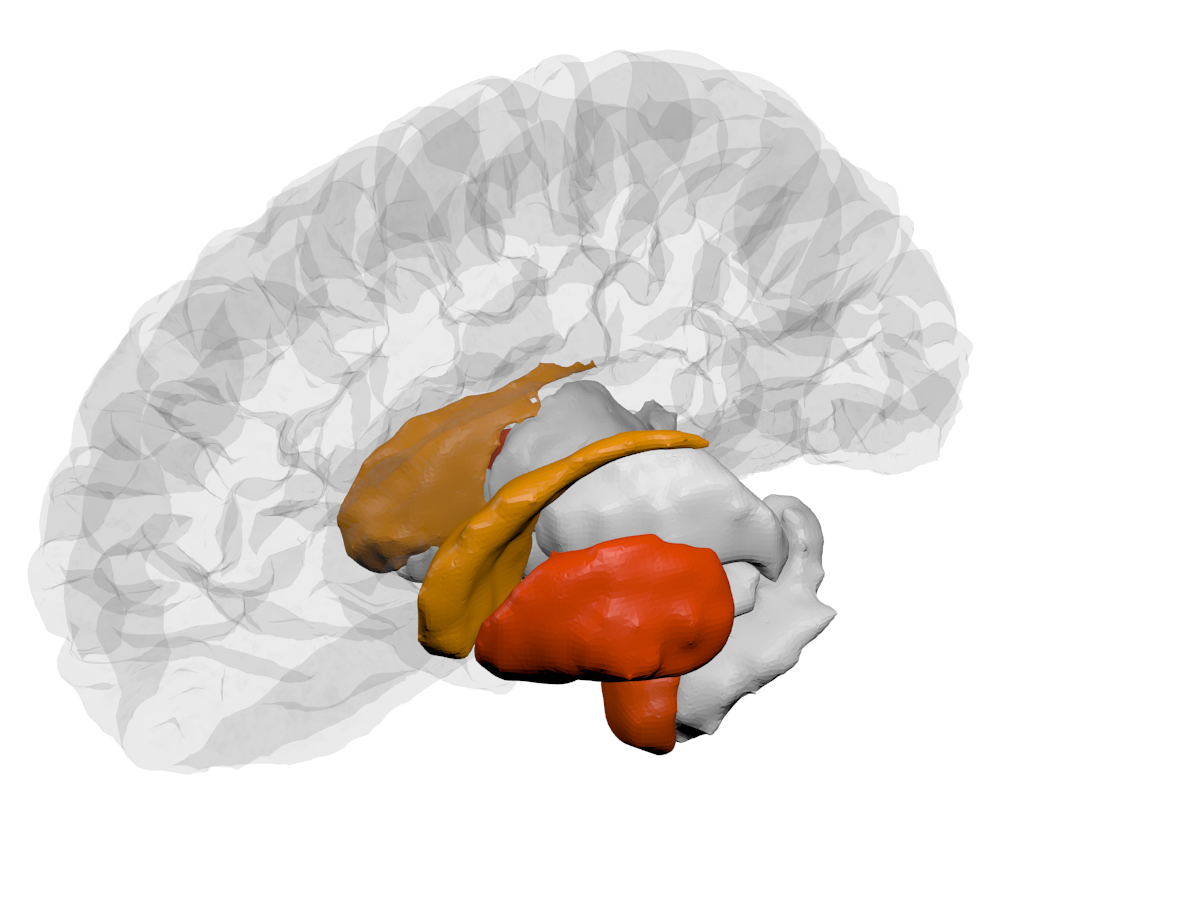
\includegraphics[height=1.5cm]{subcortical_1}
\end{subfigure}
}


\definecolor{light-gray}{gray}{0.6}



% \begin{comment}

\begin{frame}
\frametitle{About me}

\begin{itemize}
 \item Grew up in Pitesti, Romania
  \item 2010-2014: Studied a 4-year MEng in Computer Science at Imperial College London
  \item 2014-2019: PhD in Medical Imaging at UCL (with Daniel Alexander)
  \item 2019: Postdoc at MIT with Pollina Golland (working on image analysis of stroke)

  \begin{figure}
  \vspace{1em}
  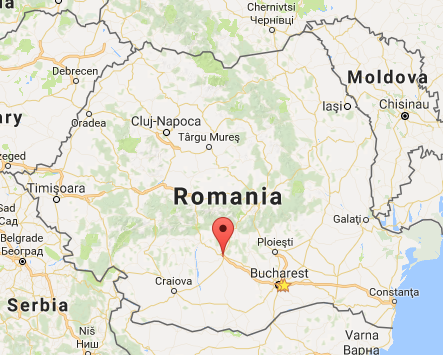
\includegraphics[height=2.5cm]{pitestiRomania}\hspace{1em}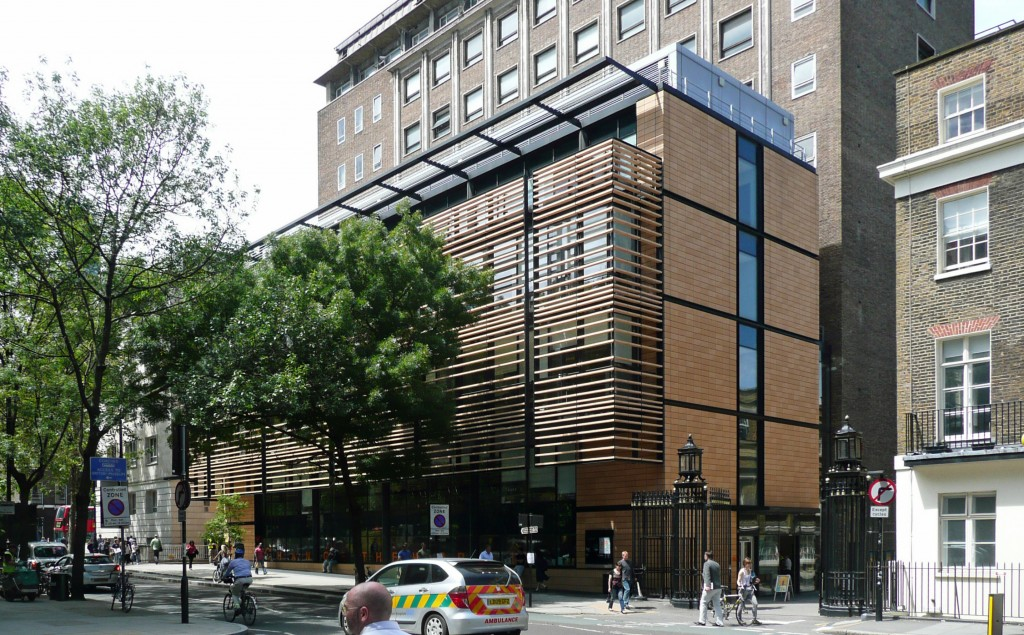
\includegraphics[height=2.5cm,trim=0 0 0 100,clip]{uclFrontEng.jpg} \hspace{1em}
  \end{figure}
 
 \vspace{1em}

 
 
  \begin{figure}
   \centering
%     \hfill
    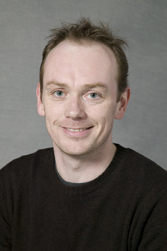
\includegraphics[height=2.5cm]{Danny-Alexander.jpeg}
    \hspace{3em}
    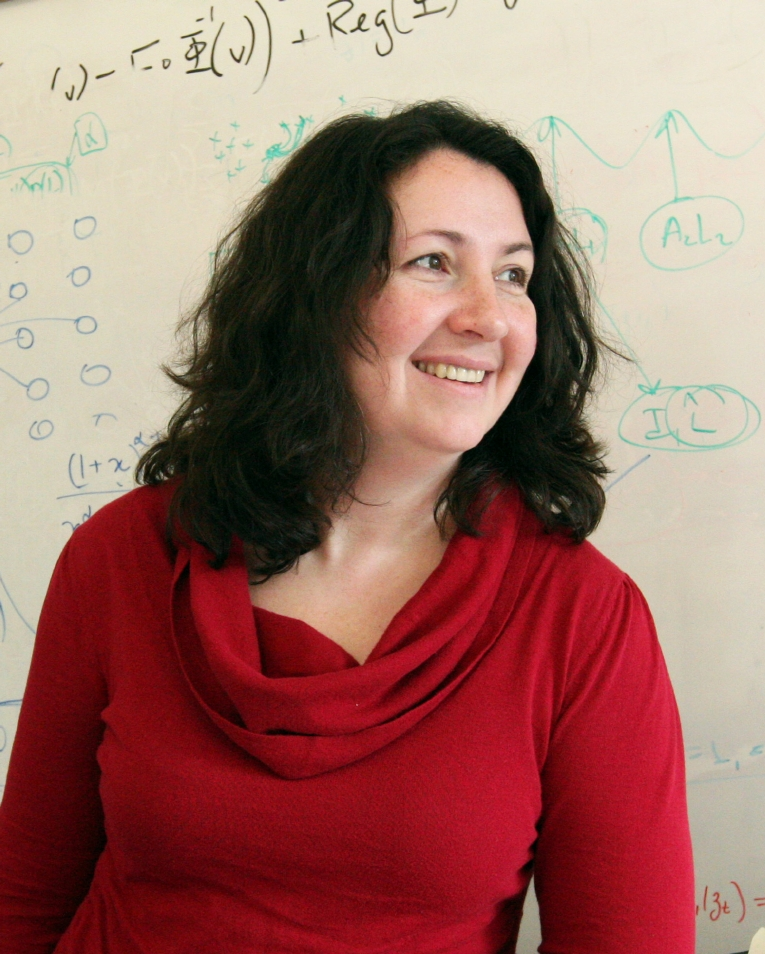
\includegraphics[height=2.5cm]{polina}  
%     \hfill
  \end{figure}



\end{itemize}

\end{frame}




\begin{frame}
\frametitle{Progression of Neurodegenerative Diseases (POND)}

\begin{figure}
\centering
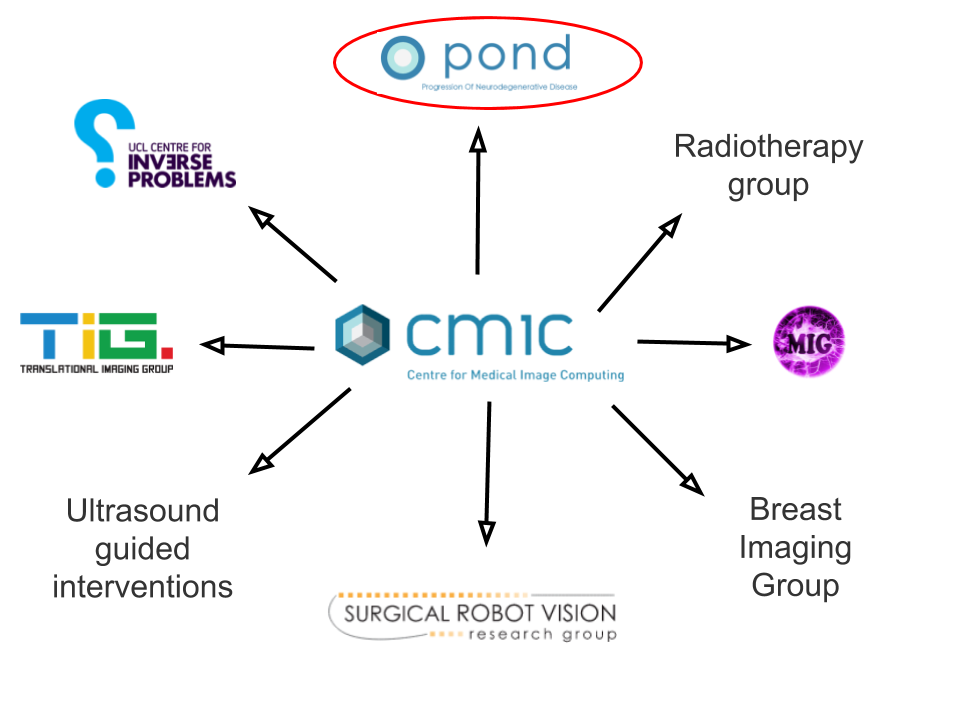
\includegraphics[height=8cm]{pond_diagram} 
\end{figure}



\end{frame}


\begin{frame}
\frametitle{POND Aim: Develop Computational Models for Disease Progression}

\newcommand{\mnpHeight}{3cm}

\vspace{-3em}
% \textbf{Background}:
% \onslide<1> \begin{itemize}
%   \item Aim: Develop computational models for disease progression
  
%   \vfill 
  
  \hspace{-2em}
  \begin{small}
  \begin{figure}[h]
  \centering
    \begin{minipage}[t][\mnpHeight][t]{0.49\linewidth}
  \centering
    \textbf{Event-Based Model}\\ \footnotesize{(Fontejin et al., Neuroimage, 2012)}\\    
    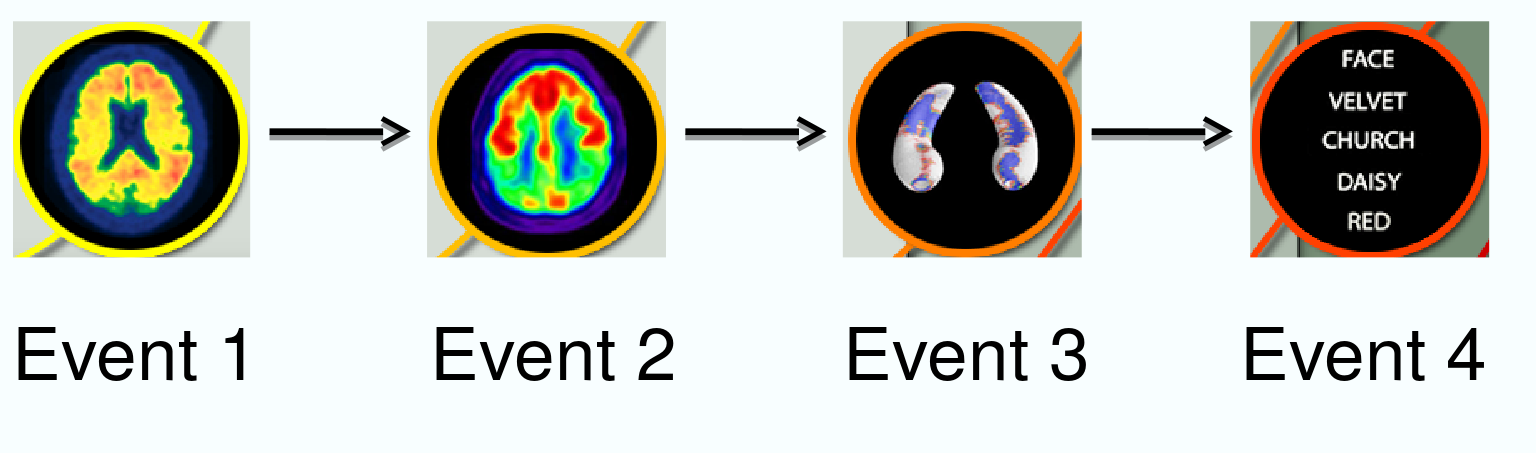
\includegraphics[width=0.9\textwidth,trim=0 0 0 0,clip]{ebm_openday}
      \vspace{1em}
%     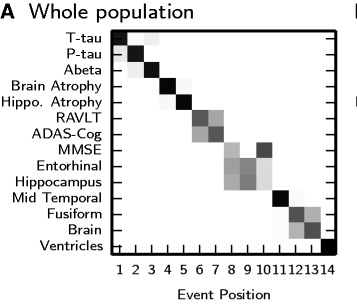
\includegraphics[width=0.4\textwidth]{young_positional_variance}
  \end{minipage}
  \begin{minipage}[t][\mnpHeight][t]{0.49\linewidth}
    \centering
    \textbf{Differential Equation Model}\\ \footnotesize{(Oxtoby et al., Brain, 2018)}
    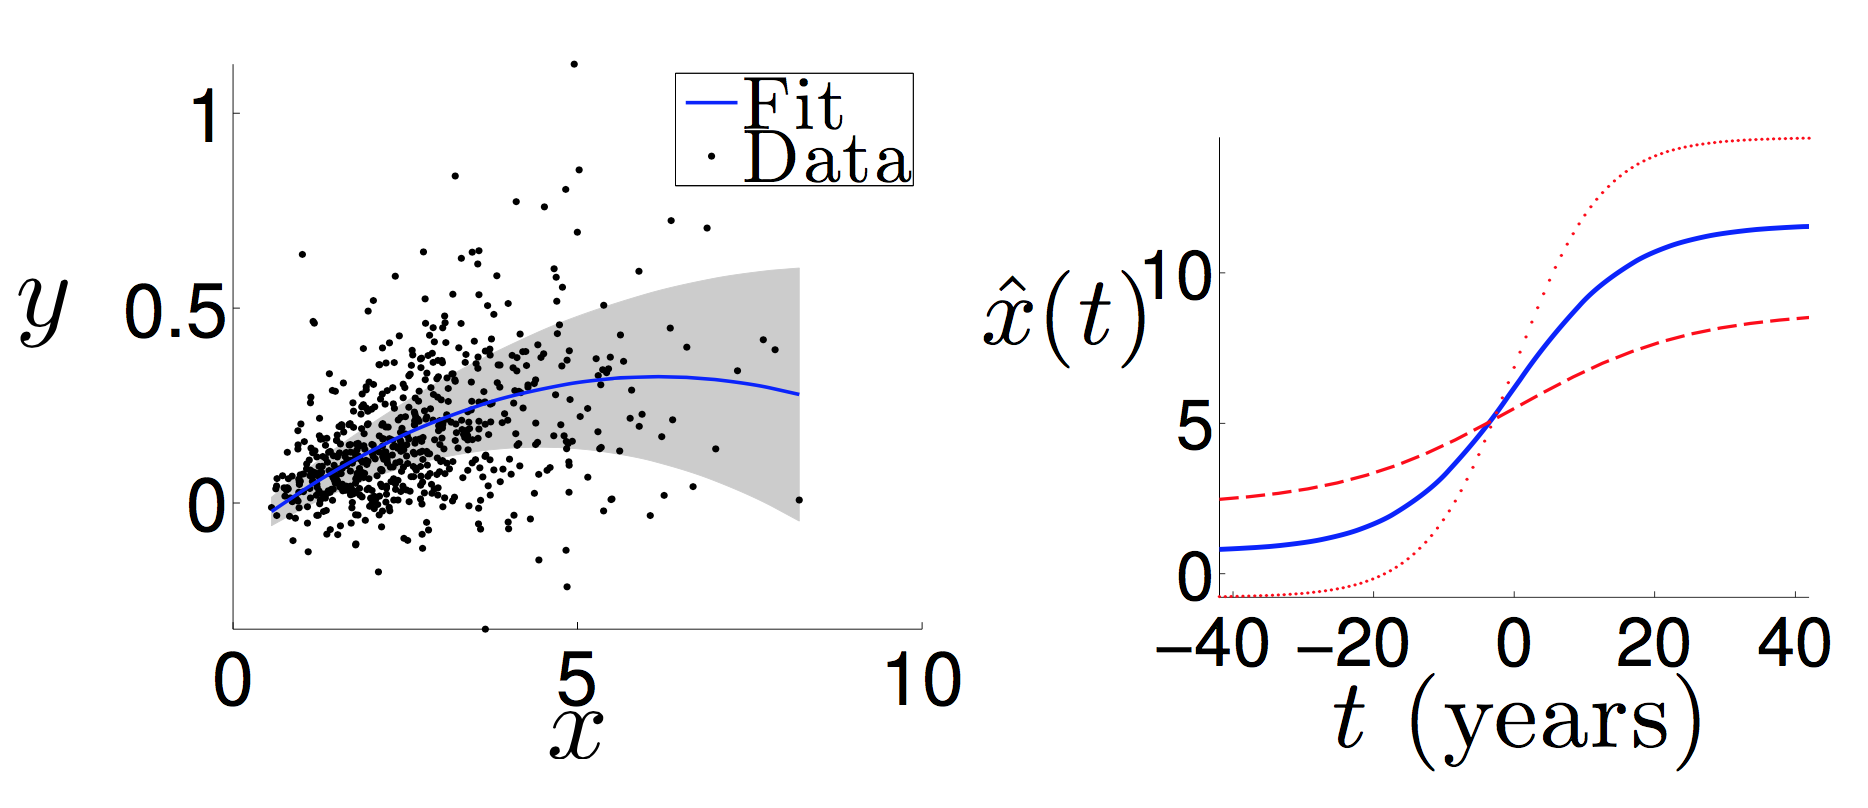
\includegraphics[width=0.9\textwidth,trim=0 0 0 0, clip]{dem_neil}
  \end{minipage}

  \vspace{2em}
  \begin{minipage}[t][\mnpHeight][t]{0.49\linewidth}
    \centering
    \textbf{Gaussian-Process Regression}\\ \footnotesize{(Lorenzi et al., IPMI, 2015)}
    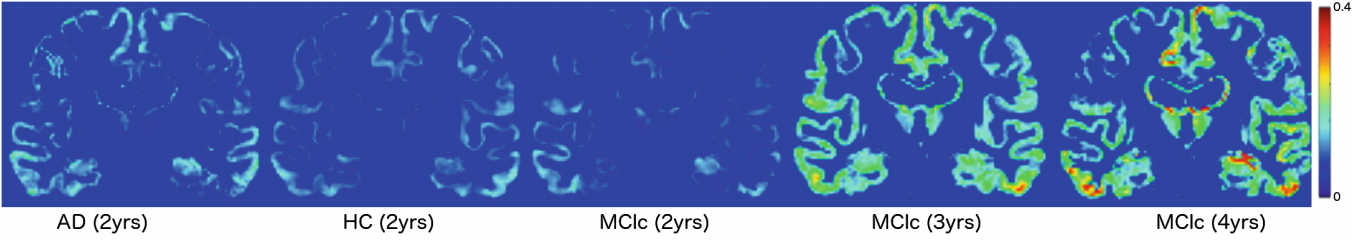
\includegraphics[width=0.9\textwidth,trim=0 0 0 0, clip]{lorenzi_ipmi2015}
    
    \vspace{2em}
    
  \end{minipage}
  \begin{minipage}[t][\mnpHeight][t]{0.49\linewidth}
    \centering
    \textbf{Subtype and Stage Inference}\\ \footnotesize{(Young et al., Nature Comms., 2018)}
    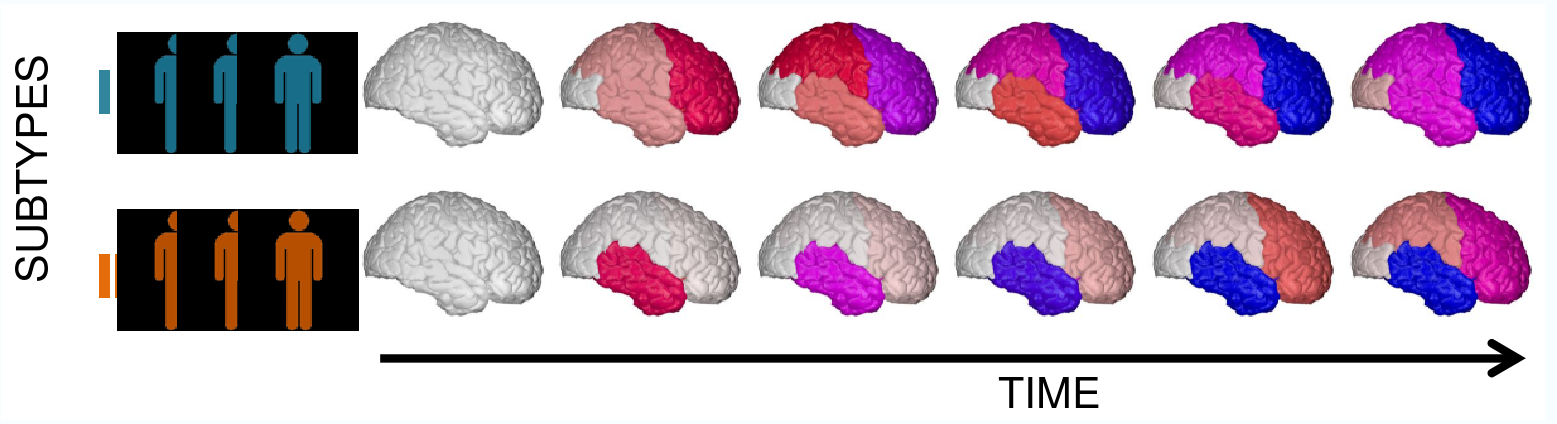
\includegraphics[width=0.9\textwidth]{sustain}
  \end{minipage}


  \end{figure}
  \end{small}
  
  \vspace{-2em}
  
% \end{itemize}


\end{frame}



\begin{frame}
\frametitle{POND Aim 2: Apply the Models to Distinct Neurodegenerative Diseases}

\newcommand{\mnpHeight}{3cm}

\vspace{-3em}
% \textbf{Background}:
% \begin{itemize}
%   \item 
  
%   \vfill 
  
  \hspace{-2em}
  \begin{small}
  \begin{figure}[h]
  \centering
  
      \begin{minipage}[t][\mnpHeight][t]{0.49\linewidth}
    \centering
    \textbf{typical AD}\\ \footnotesize{(Young et al., Nature Comms., 2018)}
    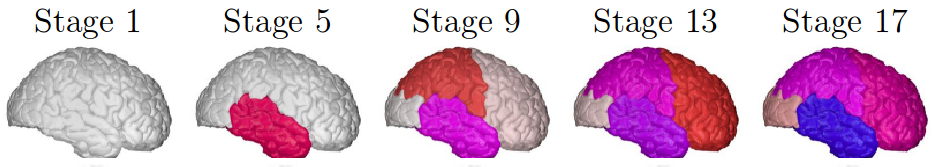
\includegraphics[width=0.9\textwidth]{young_progression.png}
  \end{minipage}
  \begin{minipage}[t][\mnpHeight][t]{0.49\linewidth}
    \centering
    \textbf{Familial AD}\\ \footnotesize{(Oxtoby et al., Brain, 2018)}
    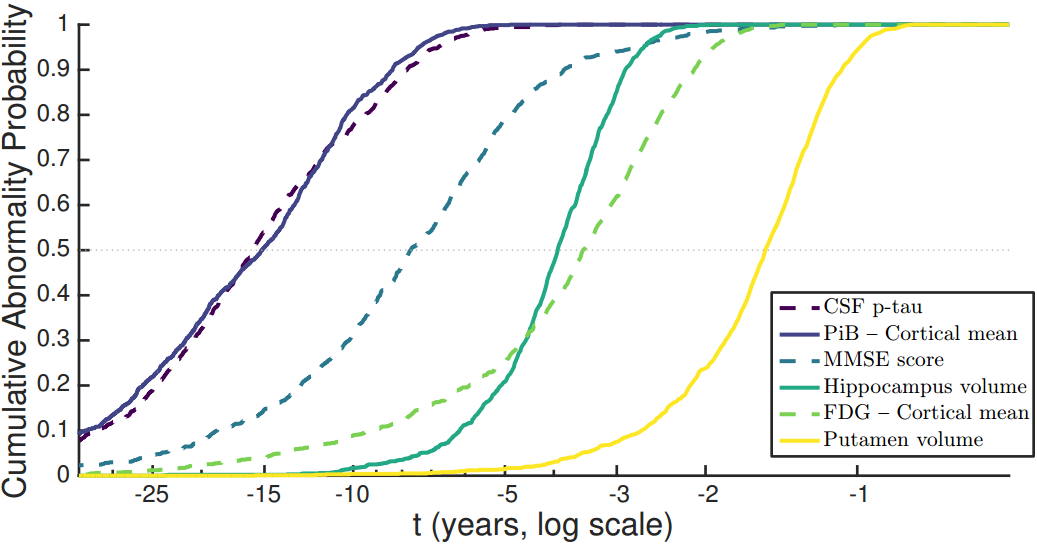
\includegraphics[width=0.7\textwidth,trim=0 0 0 0, clip]{neil_dian.png}
    
    \vspace{2em}
    
  \end{minipage}
  \vspace{2em}
  
    \begin{minipage}[t][\mnpHeight][t]{0.49\linewidth}
  \centering
    \textbf{Multiple sclerosis}\\ \footnotesize{(Eshaghi et al., Brain, 2017)}\\    
    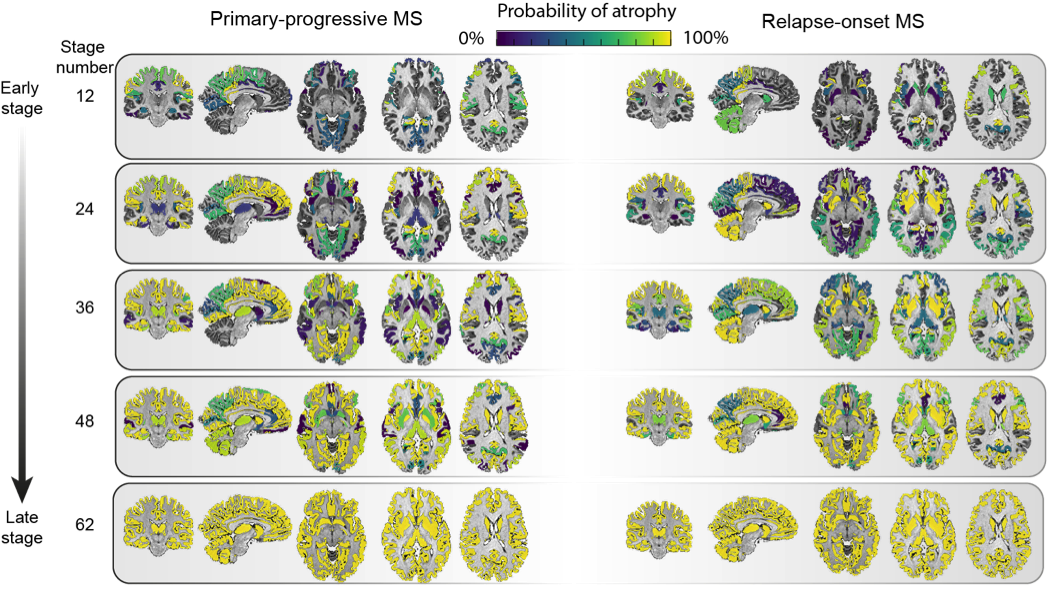
\includegraphics[width=0.9\textwidth,trim=0 0 0 0,clip]{ms_arman}
      \vspace{1em}
%     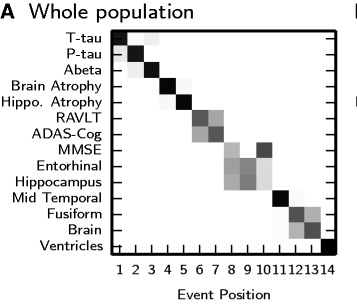
\includegraphics[width=0.4\textwidth]{young_positional_variance}
  \end{minipage}
  \begin{minipage}[t][\mnpHeight][t]{0.49\linewidth}
    \centering
    \textbf{Huntington's disease}\\ \footnotesize{(Wijeratne et al., Ann. Clin. Neurol;, 2018)}
    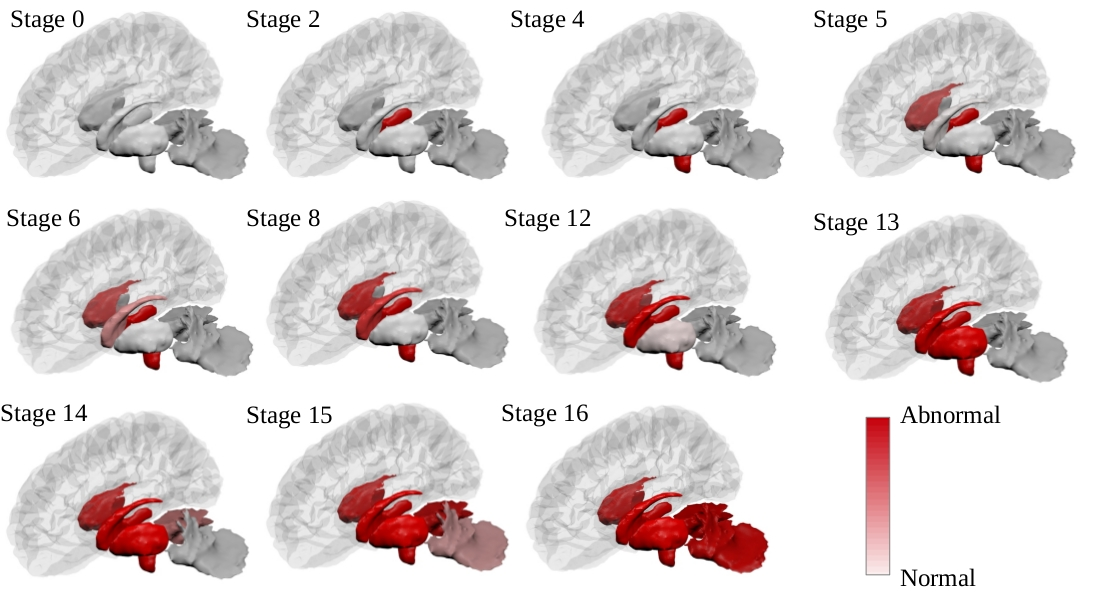
\includegraphics[width=0.9\textwidth,trim=0 0 0 0, clip]{hd_peter}
  \end{minipage}

\end{figure}
  \end{small}
  
%   \vspace{-2em}
  
% \end{itemize}



\end{frame}


\newcommand{\titleHigh}[1]{{\transparent{1.0}\textbf{#1}}} % title highlighting
\newcommand{\titleHighTwo}[1]{\underline{\textbf{#1}}} % title highlighting 2
\newcommand{\transpLevel}{0.4}

% \begin{frame}
% \frametitle{\textcolor{red}{Disease Progression} \textcolor{green}{Modelling} of \textcolor{blue}{Alzheimer's Disease} \textcolor{orange}{Subtypes}}
% 
% Title breakdown:\\
% \vspace{1em}
% \large{
% \textcolor{red}{Disease Progression} \textcolor{green}{Modelling} of \titleHighTwo{\textcolor{blue}{Alzheimer's Disease}} \textcolor{orange}{Subtypes}
% }
% 
% \vfill
% \vfill
% \vfill
% 
% \end{frame}



\begin{frame}
\frametitle{My PhD Aim}

\begin{enumerate}
 \item Study the progression of atrophy in two diseases (using existing models): 
 \begin{itemize}
  \item typical Alzheimer's Disease (tAD)
  \item Posterior Cortical Atrophy (PCA)
 \end{itemize}
 
  \begin{figure}
  \centering
  \vspace{1em}
  \includegraphics[width=0.8\textwidth]{\epsrcPresLoc/brain_progression_16082017.png}
  \end{figure}
 
 \vspace{1em}

 \item Develop novel disease progression models (DPMs)
  \begin{equation}
  \resizebox{0.8\columnwidth}{!}{% 
  $p(X|S) = \prod_{j=1}^J \left[ \sum_{k=0}^N p(k) \left( \prod_{i=1}^k p\left(x_{s(i),j} | E_{s(i)} \right) \prod_{i=k+1}^N p\left(x_{s(i),j} | \neg E_{s(i)}\right) \right) \right]$
  }
  \end{equation}

%  \item Evaluate the performance of DPMs

\end{enumerate}

\end{frame}


\begin{frame}
\frametitle{Alzheimer's Disease is a Devastating Disease}

\vspace{-1em}
\begin{itemize}
 \item 46 million people affected worldwide
 
  \begin{figure}
 \centering
%   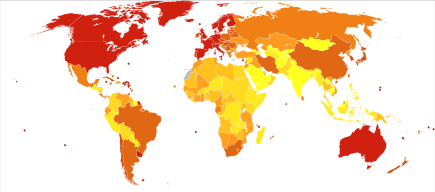
\includegraphics[height=3cm]{adPrelavence}
  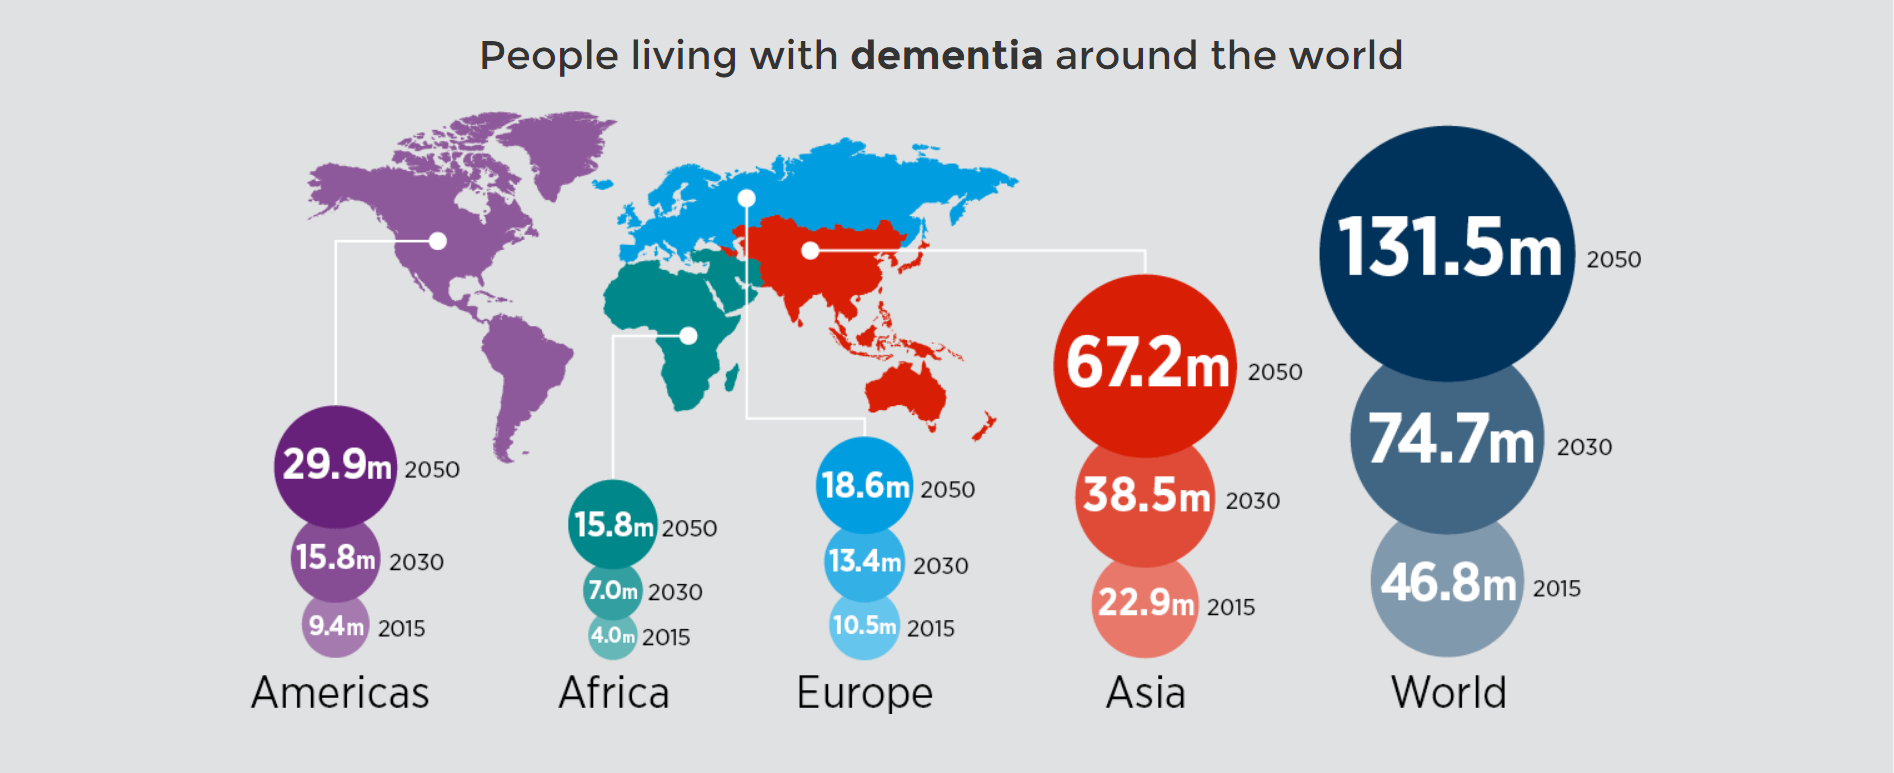
\includegraphics[height=4cm]{adPrevalanceIncreasing}
 \end{figure}
 
 \onslide<2-> \item No treatments available that stop or slow down cognitive decline
 \onslide<2-> \item Q: Why did clinical trials fail? A: Treatments were not administered early enough 
 \vspace{1em}
 \onslide<3-> \item Q: How can we then identify subjects \textbf{early} in order to administer treatments? 
 \onslide<3-> \item A: Biomarkers ...
 


 
%  \item Many known AD biomarkers:
% 
% 
% % \vspace{-1em}
% \begin{figure}
% \centering
% 
% \begin{subfigure}{0.31\textwidth}
% \centering
% Cognitive tests\\
% 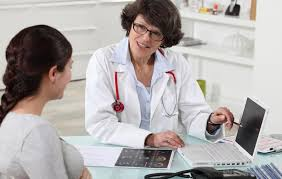
\includegraphics[height=2cm]{cogAssessment}
% \end{subfigure}
% \begin{subfigure}{0.31\textwidth}
% \centering
% Atrophy (MRI)\\
% 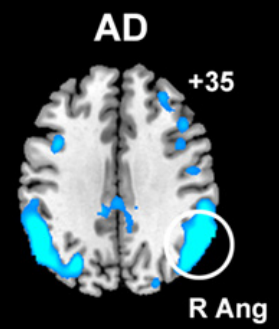
\includegraphics[height=2cm]{seeley_2009_topleft.png}
% \end{subfigure}
% \begin{subfigure}{0.31\textwidth}
% \centering
% % \vspace{1em}
% Hypometabolism (FDG PET)\\
% 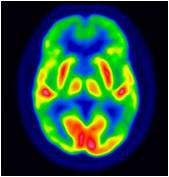
\includegraphics[height=2cm]{brainFDG}
% \end{subfigure}
% 
% 
% \vspace{1em}
% \begin{subfigure}{0.47\textwidth}
% \centering
% Tau aggregation (CSF, AV1451 PET)\\
% \includegraphics[height=2cm]{TANGLES_HIGH.jpg}
% \end{subfigure}
% \begin{subfigure}{0.47\textwidth}
% \centering
% % \vspace{1em}
% Amyloid misfolding (CSF, AV45 PET)\\
% 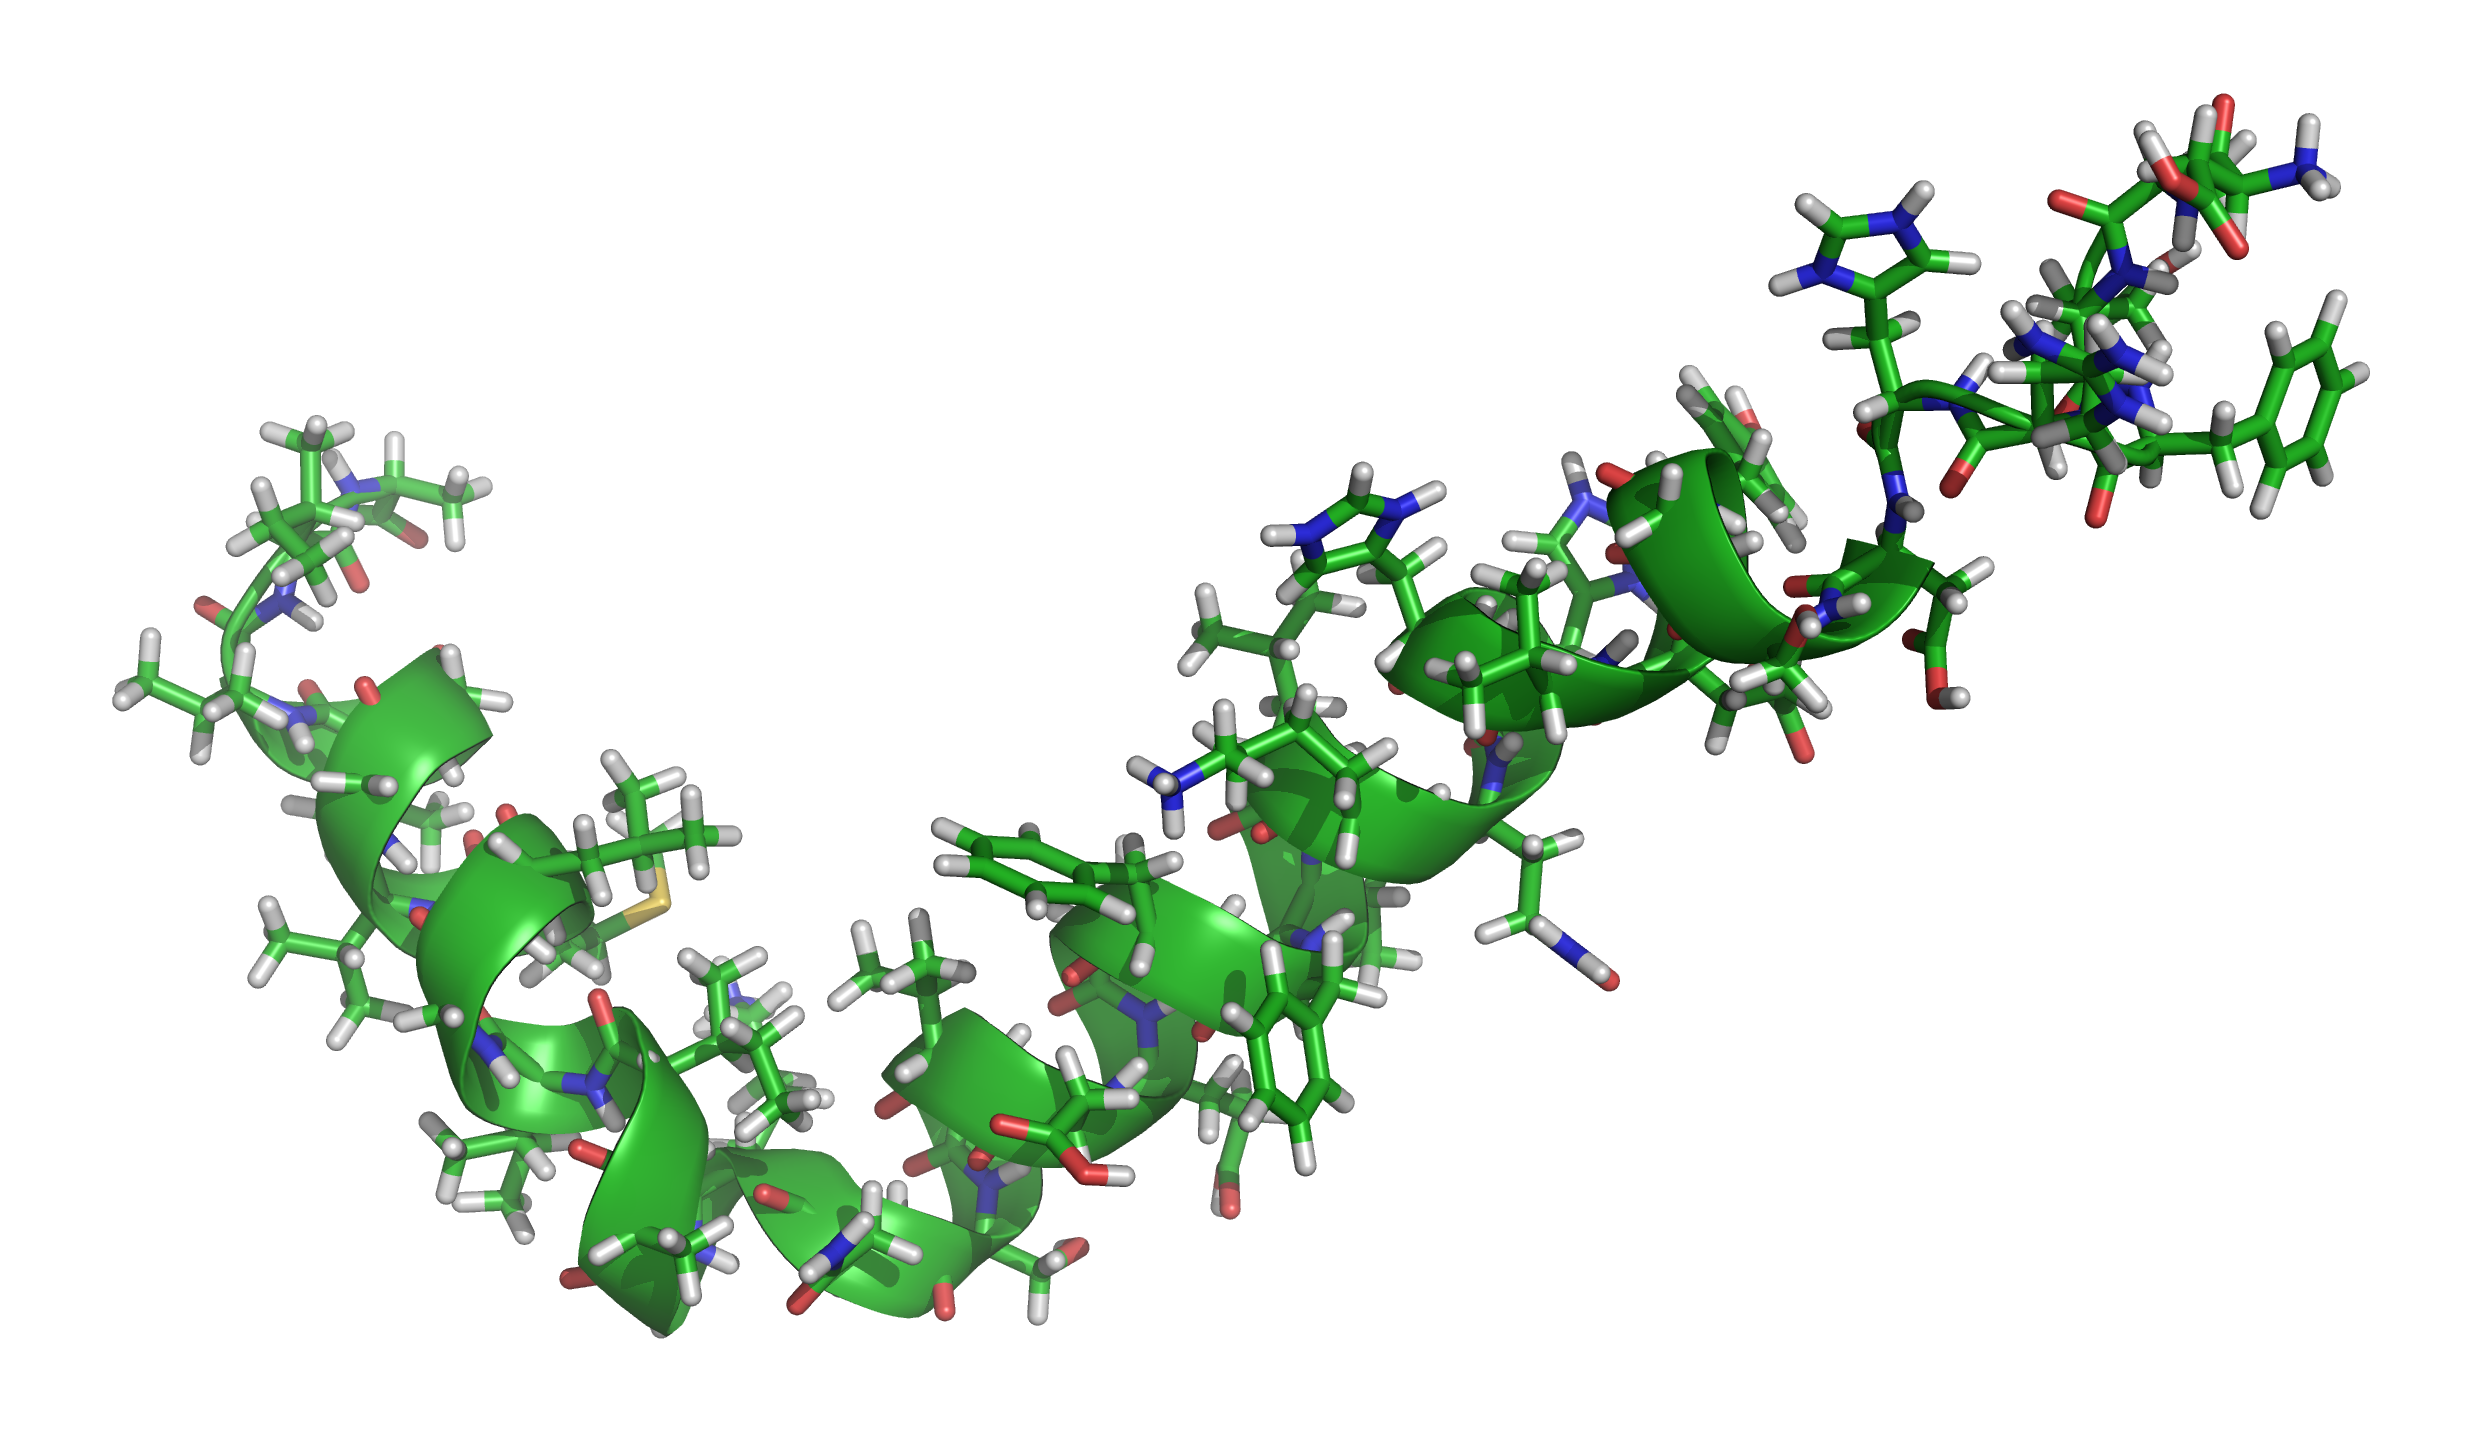
\includegraphics[height=2cm]{amyloid_beta.png}
% \end{subfigure}
% 
% 
% 
% 
% \end{figure}



\end{itemize}

\vspace{-1em}

\end{frame}

% Also say that we cannot build the model on age
\begin{frame}
\frametitle{Biomarker Evolution creates a Unique Disease Signature\\
that can be used for Staging Individuals in Clinical Trials}
% explain what are the challenges

\begin{figure}
\centering 
\vspace{1em}
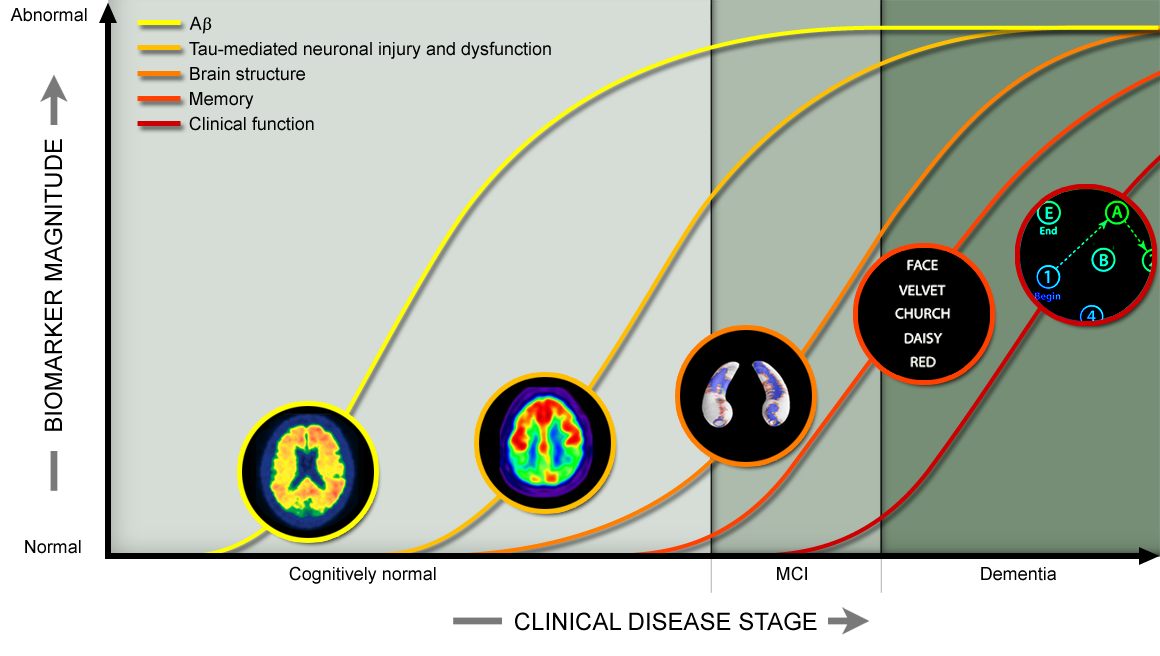
\includegraphics[height=5cm]{adniDiseaseProgression}
\hspace{-4em}ADNI website 

\end{figure}


\begin{itemize}
 \item Accurate disease staging $\rightarrow$ better patient stratification
 \item Problem: This is a "hypothetical" (i.e. qualitative) disease progression model
 \item Why construct a quantitative model? 
\end{itemize}

\end{frame}


\section{Disease Progression Modelling}

% \begin{frame}
% \frametitle{\textcolor{red}{Disease Progression} \textcolor{green}{Modelling} of \textcolor{blue}{Alzheimer's Disease} \textcolor{orange}{Subtypes}}
% 
% Title breakdown:\\
% \vspace{1em}
% \large{
% \titleHighTwo{\textcolor{red}{Disease Progression} \textcolor{green}{Modelling}} of \textcolor{blue}{Alzheimer's Disease} \textcolor{orange}{Subtypes}
% }
% 
% \vfill
% \vfill
% \vfill
% 
% \end{frame}

\begin{frame}
\frametitle{Benefits of Quantitative Disease Progression Models}

\begin{overprint}
 \onslide<1>\begin{figure}
 \centering
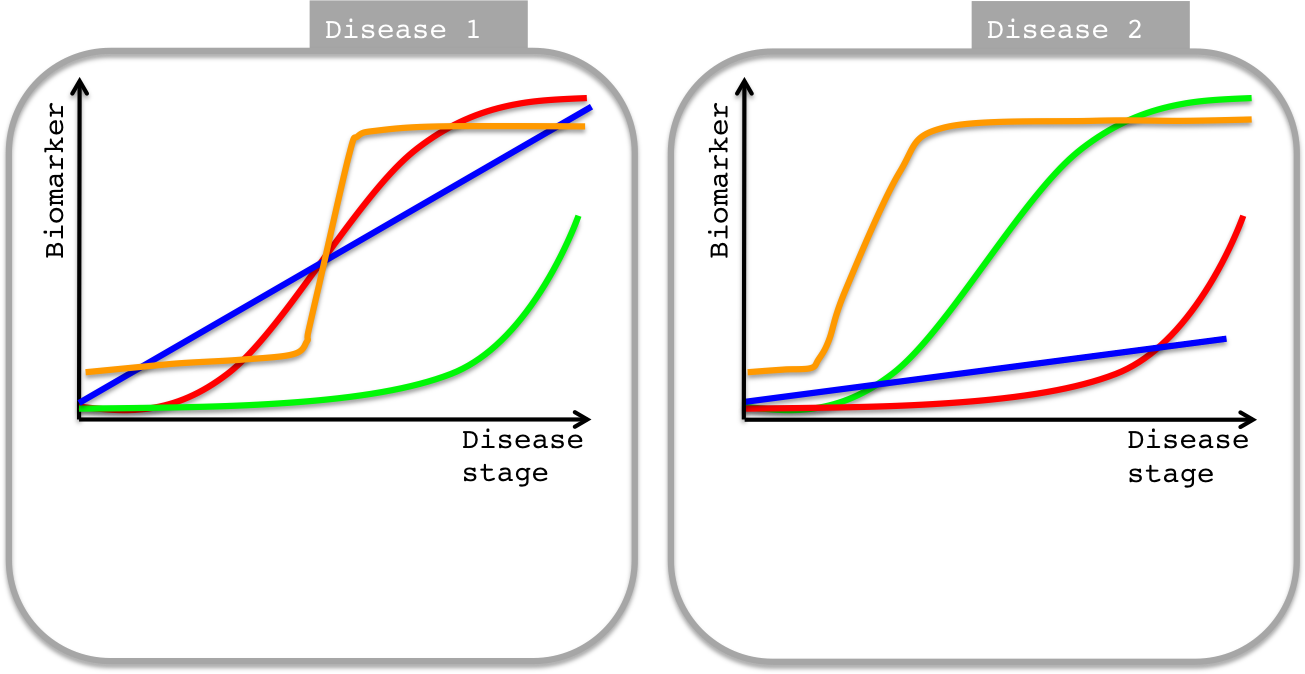
\includegraphics[height=5cm,trim=0 0 650 0,clip]{dpmDiffDiag1.png}
\end{figure}

\onslide<2> \begin{figure}
 \centering
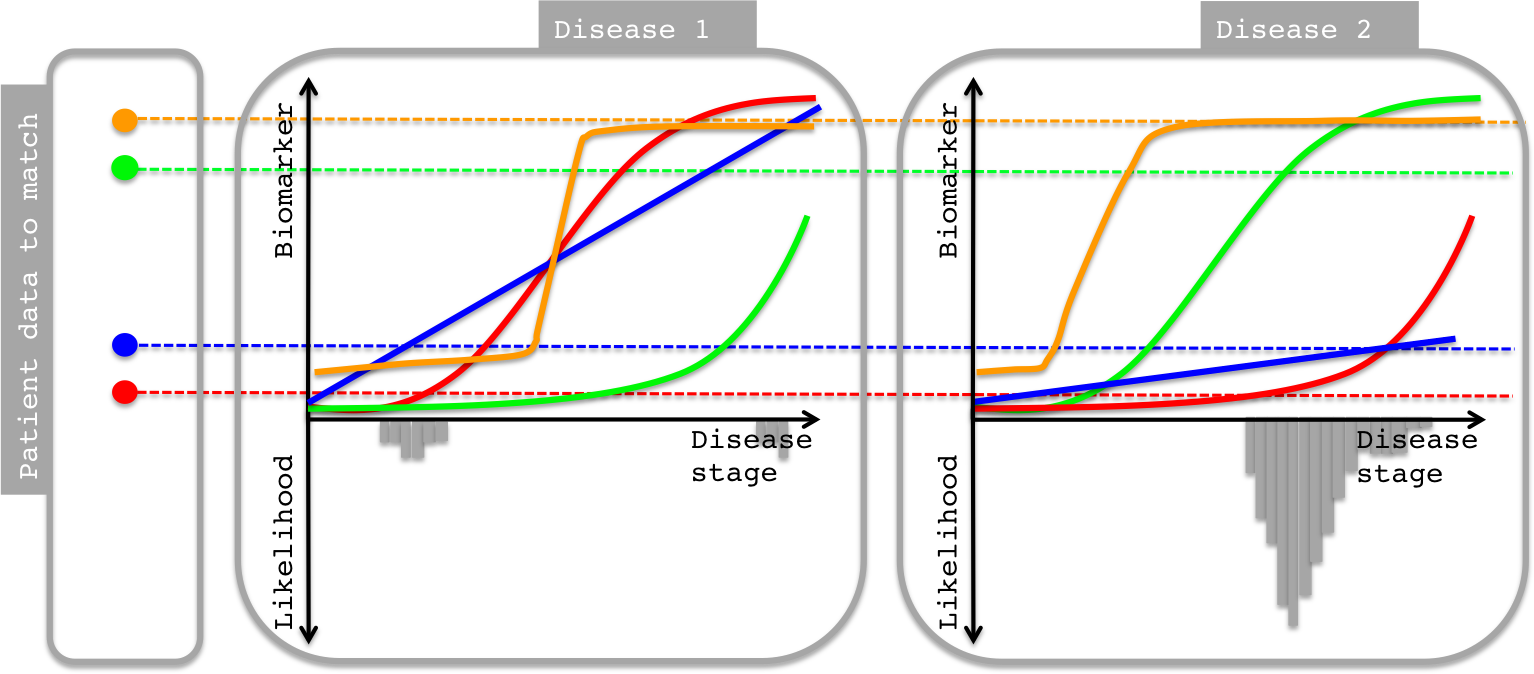
\includegraphics[height=5cm,trim=0 0 650 0,clip]{dpmDiffDiag2.png}
\end{figure}

\onslide<3-> \begin{figure}
 \centering
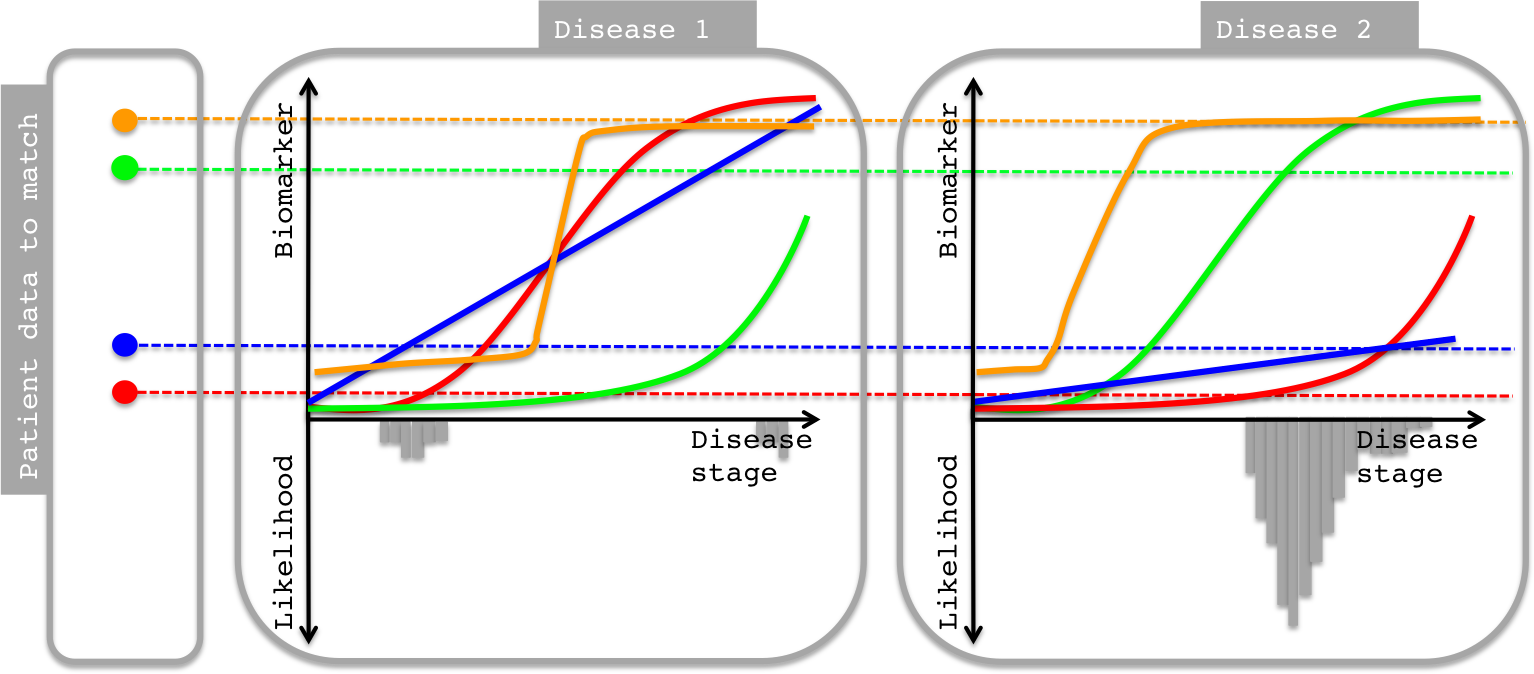
\includegraphics[height=5cm,trim=0 0 0 0,clip]{dpmDiffDiag2.png}
\end{figure}

\end{overprint}

\vspace{1em}
\begin{itemize}
 \onslide<1-> \item Basic biological insight
 \onslide<2-> \item Staging can help stratification in clinical trials
 \onslide<3-> \item Differential diagnosis and prognosis
 
 \vspace{1.5em}
 \onslide<4-> \item[] How can we build such a disease progression model?
\end{itemize}


 

\end{frame}

\begin{frame}
\frametitle{Building a Quantitative Disease Progression Model is difficult}
% explain what are the challenges

% \begin{itemize}
%  \item Using mathematical models to quantitatively estimate disease progression
% \end{itemize}

\newcommand{\heiFig}{3.5cm}
\vspace{-3em}
\begin{figure}
\centering 
% \vspace{1em}
\begin{overprint}
\onslide<1> \begin{center} \includegraphics[height=\heiFig]{\diffEqModelFld/demDiagramPlots/spaggeti_fig1.png} \end{center}
\onslide<2-3> \begin{center} \begin{tikzpicture}[scale=1,auto,swap]
    % the two brain figures on top
    \node (fig2) at (-3,0) {\includegraphics[height=\heiFig,trim=0 0 40 0,clip]{\diffEqModelFld/demDiagramPlots/spaggeti_fig2.png}};
    \node (desc2) at (fig2.north) {what we have};
    \node (fig1) at (3,0) {\includegraphics[height=\heiFig]{\diffEqModelFld/demDiagramPlots/spaggeti_fig1.png}};
    \node (desc1) at (fig1.north) {what we want};
%     \draw[line width=1, color=black,->] (fig2.east) -- node[above] {Model} ++ (fig1.west);
%     \draw[line width=0.8, color=black,->] (fig2.east) -- node[above] {Model} (fig1.west);
    
 \end{tikzpicture}
 \end{center}
 
 \onslide<4> \begin{center} \begin{tikzpicture}[scale=1,auto,swap]
    % the two brain figures on top
    \node (fig2) at (-3,0) {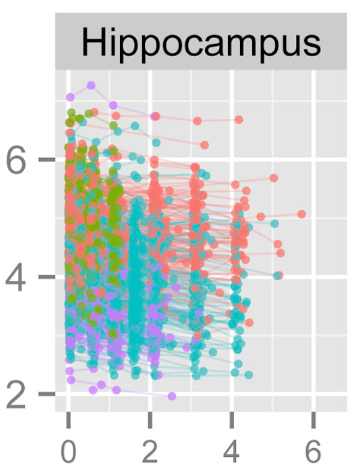
\includegraphics[height=\heiFig]{spaggeti_plot.png}};
    \node (fig1) at (3,0) {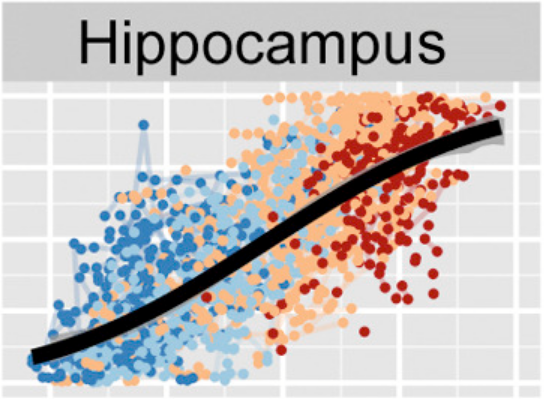
\includegraphics[height=2.5cm]{spaggeti_aligned.png}};
%     \draw[line width=1, color=black,->] (fig2.east) -- node[above] {Model} ++ (fig1.west);
%     \draw[line width=0.8, color=black,->] (fig2.east) -- node[above] {Model} (fig1.west);
    
 \end{tikzpicture}
 \end{center}
 
 \onslide<5> \begin{center} \begin{tikzpicture}[scale=1,auto,swap]
    % the two brain figures on top
    \node (fig2) at (-3,0) {\includegraphics[height=\heiFig,trim=0 0 40 0,clip]{\diffEqModelFld/demDiagramPlots/spaggeti_fig2.png}};
    \node (fig1) at (3,0) {\includegraphics[height=\heiFig]{\diffEqModelFld/demDiagramPlots/spaggeti_fig1.png}};
%     \draw[line width=1, color=black,->] (fig2.east) -- node[above] {Model} ++ (fig1.west);
%     \draw[line width=0.8, color=black,->] (fig2.east) -- node[above] {Model} (fig1.west);
    
 \end{tikzpicture}
 \end{center}
 
\onslide<6-> \begin{center} \begin{tikzpicture}[scale=1,auto,swap]
    % the two brain figures on top
    \node (fig2) at (-3,0) {\includegraphics[height=\heiFig,trim=0 0 40 0,clip]{\diffEqModelFld/demDiagramPlots/spaggeti_fig2.png}};
    \node (fig1) at (3,0) {\includegraphics[height=\heiFig]{\diffEqModelFld/demDiagramPlots/spaggeti_fig1.png}};
%     \draw[line width=1, color=black,->] (fig2.east) -- node[above] {Model} ++ (fig1.west);
    \draw[line width=0.8, color=black,->] (fig2.east) -- node[above] {Model} (fig1.west);
 \end{tikzpicture}
 \end{center}
\end{overprint}
\end{figure}

\onslide<2-> Challenges:
\begin{itemize}
 \onslide<2-> \item Patients are at unknown disease stages
 \onslide<3-> \item X-axis are not the same (need to construct the disease stage axis)
 \onslide<7-> \item Biomarkers have different trajectory shapes
 \onslide<7-> \item Cohort is heterogenous
 \onslide<7-> \item Control population not well defined
\end{itemize}
\vspace{1em}

\end{frame}




\begin{frame}[label=current]
\frametitle{My PhD Contributions}

\begin{figure}
\centering


\ovEBM
\ovVWDPM

\ovDKT
\ovTadpole

\ovPainter

\end{figure}

\end{frame}



\begin{frame}
\frametitle{Overview}

%% new slide

\begin{figure}
\centering

\ovEBM
{\transparent{0.4}
\ovVWDPM

\ovDKT
\ovTadpole

\ovPainter
}

\end{figure}
\end{frame}


\section{Cross-sectional Modelling}

\begin{frame}
\frametitle{\textbf{Clinical question}: Find the order in which GM regions become atrophied 
\begin{itemize}
 \item in PCA 
 \item in tAD
\end{itemize}
\vspace{-1.2em}
}
% discuss the hypotheses on PCA and tAD



% \vspace{2em}

\textbf{Why?} No previous studies modelled disease progression in PCA

\vspace{2em}
\textbf{Demographics}:
\begin{itemize}
 \item cohort from the Dementia Research Centre with uniquely large PCA population (70)
 
\par{\footnotesize
\rowcolors{1}{blue2}{white}
\begin{table}
\centering
\begin{tabular}{ c |C{1.2cm} | C{0.7cm} | C{1.5cm} | C{1.5cm}}% | C{1.5cm}} 
 & \textbf{\# Subjects} & \textbf{Gender} \hspace{1cm} M/F & \textbf{Age at baseline} \hspace{1cm} (years) & \textbf{Years from onset} (years)\\% & \textbf{Number of scans}\\
\textbf{Controls} & 89 & 33/56 & 60.5 $\pm$ 11 & -\\% & 2.2 $\pm$ 1.3\\ 
\textbf{PCA} & 70 & 27/43 & 63.0 $\pm$ 7 & 4.4 $\pm$ 2.8\\% & 2.4 $\pm$ 1.4\\ 
\textbf{AD} & 65 & 34/31 & 66.3 $\pm$ 8 & 4.8 $\pm$ 2.6\\% & 2.1 $\pm$ 1.3\\ 
\end{tabular}
% \caption[Baseline population demographics for DRC data]{Baseline population demographics for the DRC cohort.}
% \label{tab:drc_demographics}
\end{table}
}
\end{itemize}

\textbf{Data}: Structural MRI scans\\

\vspace{1em}


\vspace{1em}
\textbf{How?} The Event-Based Model ...

\end{frame}

% TODO: add label with informative snapshot
\begin{frame}
\frametitle{Key Idea: The Event-Based Model Estimates an Atrophy Sequence from\\ Informative Patient Snapshots}

\vspace{-2em}
\begin{itemize}
 \item Event-Based Model (EBM): Fontejin et al., Neroimage, 2012.
 \item Aim: Region 1 $\rightarrow$ Region 2 vs Region 2 $\rightarrow$ Region 1
\end{itemize}

\vspace{1em}
\begin{figure}
\begin{tikzpicture}

\onslide<1->{
\node (tab1) at (-3,2.5) {
\begin{tabular}{c | c | c | c}
& Patient 1 & Patient 2 & Patient 3\\
\hline
  Region 1 & 1.1 & 0.9 & 0.1\\
  Region 2 & 0.95 & 0.0 & 0.05\\ 
\end{tabular}
};
}

\onslide<2->{
\node (tab2) at (3,2.5) {
\begin{tabular}{c | c | c | c}
& Patient 1 & Patient 2 & Patient 3\\
\hline
  Region 1 & \textcolor{green!60!black}{normal} & \textcolor{green!60!black}{normal} & \textcolor{red}{abnormal}\\
  Region 2 & \textcolor{green!60!black}{normal} & \textcolor{red}{abnormal} & \textcolor{red}{abnormal}\\ 
\end{tabular}
};
\draw[->,line width=0.2mm] (tab1) -- (tab2);
}

\onslide<3>{
\node (mixModel) at (1.5,0) {
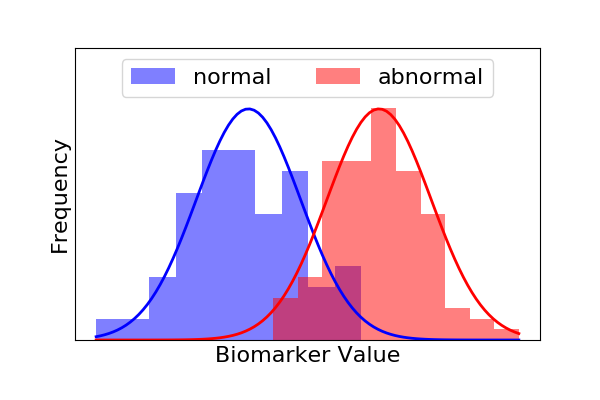
\includegraphics[height=2cm]{abnormal1.png}};
\node (mixModelLabel) at (mixModel.north) {Region 1};
\node (mixModel2) at (4.5,0) {
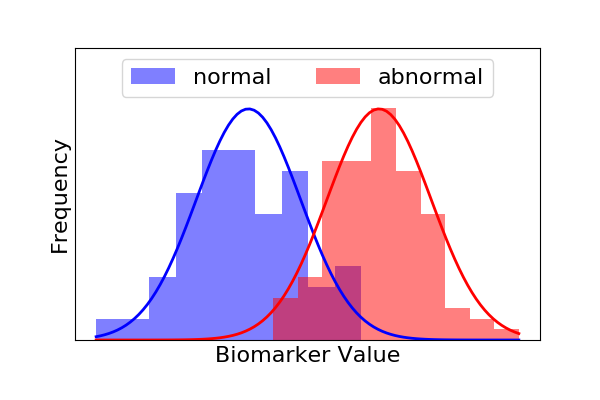
\includegraphics[height=2cm]{abnormal1.png}};
\node (mixModelLabel2) at (mixModel2.north) {Region 2};
}  
  
\onslide<4->{
\node (seq) at (3,0) {Estimated Sequence: Region 2 $\rightarrow$ Region 1};
\node (seqDummyUp) at (3,0.5) {};
\draw[->,line width=0.2mm] (tab2) -- (seqDummyUp);
}

\onslide<5->{
\node (fig1) at (-2.5,0) {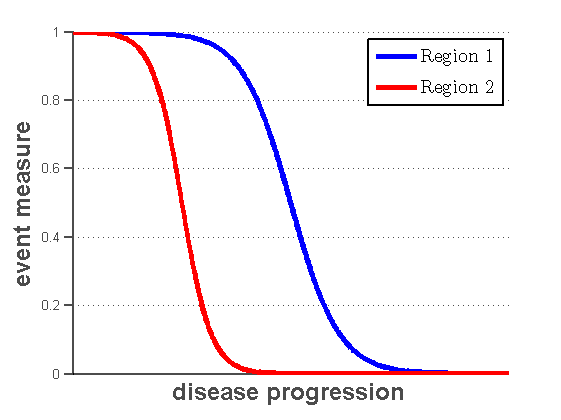
\includegraphics[height=3.0cm]{ebmMethod2Biomk}}; 
\draw[-,line width=0.4mm,] (-3.75,2) -- (-3.75,-1.5);
\draw[-,line width=0.4mm,] (-2.4,2) -- (-2.8,1.5) -- (-2.8,-1.5);
\draw[-,line width=0.4mm,] (-1.1,2) -- (-1.9,1.5) -- (-1.9,-1.5);
}

\end{tikzpicture}


\end{figure}

\end{frame}


\begin{frame}[label=current]
\frametitle{The EBM assumes a subject at stage $k$ has first $k$ biomarkers \textcolor{red}{"abnormal"} and the last $N-k$ biomarkers \textcolor{green!60!black}{"normal"}}

\begin{itemize}
%  \item Finds the most likely abnormality (i.e. atrophy) sequence using greedy ascent

 \item Evaluate data likelihood under normal and abnormal distributions:
 \begin{itemize}
  \item normal - $\textcolor{green!60!black}{ p\left(x_{s(i),j} | \neg E_{s(i)}\right) }$
  \item abnormal - $\textcolor{red}{p\left(x_{s(i),j} | E_{s(i)} \right)}$
 \end{itemize}
 
 \item Compute likelihood of one subject $j$ being at stage $k$ given sequence $S$:
 \begin{align*}
& p(X_j|S,k) = \prod_{i=1}^k \textcolor{red}{p\left(x_{s(i),j} | E_{s(i)} \right)} \prod_{i=k+1}^N \textcolor{green!60!black}{ p\left(x_{s(i),j} | \neg E_{s(i)}\right) } 
 \end{align*}

 
 \item Marginalise stage $k$:
 
 $$p(X_j|S) =  \sum_{k=0}^N p(k) \left( \prod_{i=1}^k \textcolor{red}{p\left(x_{s(i),j} | E_{s(i)} \right)} \prod_{i=k+1}^N \textcolor{green!60!black}{ p\left(x_{s(i),j} | \neg E_{s(i)}\right) } \right) $$
  
 \item Extend to all subjects:
$$p(X|S) = \prod_{j=1}^J \left[ \sum_{k=0}^N p(k) \left( \prod_{i=1}^k \textcolor{red}{p\left(x_{s(i),j} | E_{s(i)} \right)} \prod_{i=k+1}^N \textcolor{green!60!black}{ p\left(x_{s(i),j} | \neg E_{s(i)}\right) } \right) \right]$$

 \item Sequence and uncertainty estimated with MCMC sampling
\end{itemize}

\end{frame}


\newcommand{\scaleBrainImg}{0.15}
\newcommand{\scaleAllSubfigsImg}{0.3}
% scale parameter for the circles and the gradient
% \tikzset{every picture/.append style={scale=0.4}}

\newcommand{\snapLocationPCA}{\pcaLongFigs/ebmSnapshotsPCA}
\newcommand{\snapLocationAD}{\pcaLongFigs/ebmSnapshotsAD}
\newcommand{\snapLocationEAR}{\pcaLongFigs/ebmSnapshotsEAR}
\newcommand{\snapLocationPER}{\pcaLongFigs/ebmSnapshotsPER}
\newcommand{\snapLocationSPA}{\pcaLongFigs/ebmSnapshotsSPA}



\makeatletter
\define@key{Gin}{pcaSubFigParams}[]{\setkeys{Gin}{trim=0 440 0 0,clip,scale=0.13}}
\makeatother

\newcommand{\scaleAllSubfigsPcaSubgrTikz}{0.25}
\newcommand{\scaleBrainImgPcaSubgr}{0.12}
\newcommand{\stageLabelFntSizePcaSubgr}[1]{\footnotesize{#1}}


\newcommand{\adEbmRes}[1]{
\begin{figure}
  \begin{subfigure}{0.7\textwidth}
  \centering
  %\begin{subfigure}[b]{0.15\textwidth}
    \begin{tikzpicture}[scale=\scaleAllSubfigsImg,auto,swap]

  % the two brain figures on top
    \node (upper_brain) at (0,1.5) { \includegraphics[scale=\scaleBrainImg,trim=0 0 240 0,clip=true]{\snapLocationAD/stage_4.eps}};
    \node (lower_brain) at (0,-1.5) { \includegraphics[scale=\scaleBrainImg,trim=240 0 0 0,clip=true]{\snapLocationAD/stage_4.eps}};
    \node[above=0cm of upper_brain] (stage) {Stage 4};
    % the balls
    
    \end{tikzpicture}
  %\end{subfigure}
  % next subfigure
  \hspace{-1.5em}
  ~
  \begin{tikzpicture}[scale=\scaleAllSubfigsImg,auto,swap]
    % the two brain figures on top
    \node (upper_brain) at (0,1.5) { \includegraphics[scale=\scaleBrainImg,trim=0 0 240 0,clip=true]{\snapLocationAD/stage_8.eps}};
    \node (lower_brain) at (0,-1.5) { \includegraphics[scale=\scaleBrainImg,trim=240 0 0 0,clip=true]{\snapLocationAD/stage_8.eps}};
    \node[above=0cm of upper_brain] (stage) {Stage 8};
    % the balls
    
    \end{tikzpicture}
  %\end{subfigure}
  % next subfigure
  \hspace{-1.5em}
  ~
  %\begin{subfigure}[b]{0.15\textwidth}
    \begin{tikzpicture}[scale=\scaleAllSubfigsImg,auto,swap]

    % the two brain figures on top
    \node (upper_brain) at (0,1.5) { \includegraphics[scale=\scaleBrainImg,trim=0 0 240 0,clip=true]{\snapLocationAD/stage_16.eps}};
    \node (lower_brain) at (0,-1.5) { \includegraphics[scale=\scaleBrainImg,trim=240 0 0 0,clip=true]{\snapLocationAD/stage_16.eps}};
    \node[above=0cm of upper_brain] (stage) {Stage 16};
    % the balls
    
    \end{tikzpicture}
  %\end{subfigure}
  % next subfigure
  \hspace{-1.5em}
  ~
  %\begin{subfigure}[b]{0.15\textwidth}
    \begin{tikzpicture}[scale=\scaleAllSubfigsImg,auto,swap]

    % the two brain figures on top
    \node (upper_brain) at (0,1.5) { \includegraphics[scale=\scaleBrainImg,trim=0 0 240 0,clip=true]{\snapLocationAD/stage_24.eps}};
    \node (lower_brain) at (0,-1.5) { \includegraphics[scale=\scaleBrainImg,trim=240 0 0 0,clip=true]{\snapLocationAD/stage_24.eps}};
    \node[above=0cm of upper_brain] (stage) {Stage 24};
    % the balls
    
    \end{tikzpicture}
  %\end{subfigure}
  % next subfigure
  \hspace{-1.5em}
  ~
  %\begin{subfigure}[b]{0.15\textwidth}
    \begin{tikzpicture}[scale=\scaleAllSubfigsImg,auto,swap]

    % the two brain figures on top
    \node (upper_brain) at (0,1.5) { \includegraphics[scale=\scaleBrainImg,trim=0 0 240 0,clip=true]{\snapLocationAD/stage_32.eps}};
    \node (lower_brain) at (0,-1.5) { \includegraphics[scale=\scaleBrainImg,trim=240 0 0 0,clip=true]{\snapLocationAD/stage_32.eps}};
    \node[above=0cm of upper_brain] (stage) {Stage 32};
    % the balls
    
    \end{tikzpicture}
  %\end{subfigure}
  % next subfigure
%   \hspace{-1.5em}
%   ~
%   %\begin{subfigure}[b]{0.15\textwidth}
%     \begin{tikzpicture}[scale=\scaleAllSubfigsImg,auto,swap]
% 
%     % the two brain figures on top
%     \node (upper_brain) at (0,1.5) { \includegraphics[scale=\scaleBrainImg,trim=0 0 240 0,clip=true]{\snapLocationAD/stage_40.eps}};
%     \node (lower_brain) at (0,-1.5) { \includegraphics[scale=\scaleBrainImg,trim=240 0 0 0,clip=true]{\snapLocationAD/stage_40.eps}};
%     \node[above=0cm of upper_brain] (stage) {Stage 40};
%     % the balls
%     
%     \end{tikzpicture}
  %\end{subfigure}
  % next subfigure
  \hspace{-1.5em}
  ~
  \hspace{1em}
  % the red-to-yellow gradient on the right
  \begin{tikzpicture}[scale=\scaleAllSubfigsImg,auto,swap]
    \shade[top color=red,bottom color=gray!30] (0,0) rectangle (0.5,5);
    \node[inner sep=0] (corr_text) at (0.2,5.5) {abnormal};
    \node[inner sep=0] (corr_text) at (0.2,-0.5) {normal};
  \end{tikzpicture}
%   \caption{Progression of brain volume loss}
%   \label{fig:SnapEBMPCAa}
  \end{subfigure}
  {#1}
%   \begin{subfigure}{1\textwidth}
%   \centering
%   \includegraphics[scale=0.35]{\pcaLongFigs/patientStagesAD}
%   \caption{Subject staging}
% %   \label{fig:SnapEBMPCAb}
%   \end{subfigure}  
  
\end{figure}
}

\newcommand{\pcaEbmRes}[1]{
\begin{figure}

  \begin{subfigure}{0.7\textwidth}
  \centering
  %\begin{subfigure}[b]{0.15\textwidth}
  

    \begin{tikzpicture}[scale=\scaleAllSubfigsImg,auto,swap]
    % the two brain figures on top
    \node (upper_brain) at (0,1.5) { \includegraphics[scale=\scaleBrainImg,trim=0 0 240 0,clip=true]{\snapLocationPCA/stage_4.eps}};
    \node (lower_brain) at (0,-1.5) { \includegraphics[scale=\scaleBrainImg,trim=240 0 0 0,clip=true]{\snapLocationPCA/stage_4.eps}};
    \node[above=0cm of upper_brain] (stage) {Stage 4};
    % the balls
    \end{tikzpicture}
  %\end{subfigure}
  % next subfigure
  \hspace{-1.5em}
  ~
    \begin{tikzpicture}[scale=\scaleAllSubfigsImg,auto,swap]

    % the two brain figures on top
    \node (upper_brain) at (0,1.5) { \includegraphics[scale=\scaleBrainImg,trim=0 0 240 0,clip=true]{\snapLocationPCA/stage_8.eps}};
    \node (lower_brain) at (0,-1.5) { \includegraphics[scale=\scaleBrainImg,trim=240 0 0 0,clip=true]{\snapLocationPCA/stage_8.eps}};
    \node[above=0cm of upper_brain] (stage) {Stage 8};
    % the balls
    
    \end{tikzpicture}
  %\end{subfigure}
  % next subfigure
  \hspace{-1.5em}
  ~
  %\begin{subfigure}[b]{0.15\textwidth}
    \begin{tikzpicture}[scale=\scaleAllSubfigsImg,auto,swap]

    % the two brain figures on top
    \node (upper_brain) at (0,1.5) { \includegraphics[scale=\scaleBrainImg,trim=0 0 240 0,clip=true]{\snapLocationPCA/stage_16.eps}};
    \node (lower_brain) at (0,-1.5) { \includegraphics[scale=\scaleBrainImg,trim=240 0 0 0,clip=true]{\snapLocationPCA/stage_16.eps}};
    \node[above=0cm of upper_brain] (stage) {Stage 16};
    % the balls
    
    \end{tikzpicture}
  %\end{subfigure}
  % next subfigure
  \hspace{-1.5em}
  ~
  %\begin{subfigure}[b]{0.15\textwidth}
    \begin{tikzpicture}[scale=\scaleAllSubfigsImg,auto,swap]

    % the two brain figures on top
    \node (upper_brain) at (0,1.5) { \includegraphics[scale=\scaleBrainImg,trim=0 0 240 0,clip=true]{\snapLocationPCA/stage_24.eps}};
    \node (lower_brain) at (0,-1.5) { \includegraphics[scale=\scaleBrainImg,trim=240 0 0 0,clip=true]{\snapLocationPCA/stage_24.eps}};
    \node[above=0cm of upper_brain] (stage) {Stage 24};
    % the balls
    
    \end{tikzpicture}
  %\end{subfigure}
  % next subfigure
  \hspace{-1.5em}
  ~
  %\begin{subfigure}[b]{0.15\textwidth}
    \begin{tikzpicture}[scale=\scaleAllSubfigsImg,auto,swap]

    % the two brain figures on top
    \node (upper_brain) at (0,1.5) { \includegraphics[scale=\scaleBrainImg,trim=0 0 240 0,clip=true]{\snapLocationPCA/stage_32.eps}};
    \node (lower_brain) at (0,-1.5) { \includegraphics[scale=\scaleBrainImg,trim=240 0 0 0,clip=true]{\snapLocationPCA/stage_32.eps}};
    \node[above=0cm of upper_brain] (stage) {Stage 32};
    % the balls
    
    \end{tikzpicture}
  %\end{subfigure}
  % next subfigure
%   \hspace{-1.5em}
%   ~
%   %\begin{subfigure}[b]{0.15\textwidth}
%     \begin{tikzpicture}[scale=\scaleAllSubfigsImg,auto,swap]
% 
%     % the two brain figures on top
%     \node (upper_brain) at (0,1.5) { \includegraphics[scale=\scaleBrainImg,trim=0 0 240 0,clip=true]{\snapLocationPCA/stage_40.eps}};
%     \node (lower_brain) at (0,-1.5) { \includegraphics[scale=\scaleBrainImg,trim=240 0 0 0,clip=true]{\snapLocationPCA/stage_40.eps}};
%     \node[above=0cm of upper_brain] (stage) {Stage 40};
%     % the balls
%     
%     \end{tikzpicture}
  %\end{subfigure}
  % next subfigure
  \hspace{-1.5em}
  ~
  \hspace{1em}
  % the red-to-yellow gradient on the right
  \begin{tikzpicture}[scale=\scaleAllSubfigsImg,auto,swap]
    \shade[top color=red,bottom color=gray!30] (0,0) rectangle (0.5,5);
    \node[inner sep=0] (corr_text) at (0.2,5.5) {abnormal};
    \node[inner sep=0] (corr_text) at (0.2,-0.5) {normal};
  \end{tikzpicture}
%   \caption{Progression of brain volume loss}
%   \label{fig:SnapEBMPCAa}
  \end{subfigure}
  {#1}
   
%   \begin{subfigure}{1\textwidth}
%   \centering
%   \includegraphics[scale=0.35]{\pcaLongFigs/patientStagesPCA}
%   \caption{Subject staging}
% %   \label{fig:SnapEBMPCAb}
%   \end{subfigure}
  
\end{figure}
}


%
\begin{frame}
\frametitle{The EBM finds a Distinct Atrophy Sequence in PCA compared to tAD}

\vspace{-2em}
\begin{itemize}
 \item PCA $\rightarrow$ early occipital and superior parietal atrophy
 \item tAD $\rightarrow$ early hippocampal and inferior temporal atrophy
\end{itemize}
\vspace{2em}

{\scriptsize

%\vspace{2em}

\definecolor{light-gray}{gray}{0.6}
\begin{picture}(1,1)
\put(15,-45){\large{PCA}}
\end{picture}
\pcaEbmRes{}
\vspace{-2em}
\begin{picture}(1,1)
\put(15,-45){\large{tAD}}
\end{picture}
\adEbmRes{}

\par}

\begin{center}
 \footnotesize{Firth*, Marinescu* and Primativo* et al., Brain (recently accepted), 2019}
\end{center}




% \textbf{Conclusion}:
% \begin{itemize}
%  \item PCA: occipital and superior parietal areas are the first to become abnormal
%  \item tAD: hippocampus and temporal areas are the first to become abnormal
% \end{itemize}


\end{frame}



%TODO: highlight stage 16, make others semi-transparent
\begin{frame}
\frametitle{Atrophy Patterns Resemble Previous Studies from the Literature}

\begin{itemize}
 \item PCA $\rightarrow$ early occipital and superior parietal atrophy
 \item tAD $\rightarrow$ early hippocampal and inferior temporal atrophy
\end{itemize}

\vspace{-1.5em}

{\scriptsize

\vspace{-3em}

\definecolor{light-gray}{gray}{0.6}
% \hspace{-4em}
\begin{picture}(1,1)
\put(5,-60){\large{PCA}}
\end{picture}
\pcaEbmRes{
\begin{subfigure}{0.14\textwidth}
\centering
Lehmann et al., 2012\\
\includegraphics[height=3cm,right]{pcaLehmannGood} 
\end{subfigure}
}

\vspace{-2em}
\begin{picture}(1,1)
\put(5,-60){\large{tAD}}
\end{picture}
\adEbmRes{
\begin{subfigure}{0.14\textwidth}
\centering
 Lehmann et al., 2012\\
\includegraphics[height=3cm,right]{adLehmannGood} 
\end{subfigure}
}

\par}

\vspace{-1em}
\hspace{6em}\footnotesize{Firth*, Marinescu* and Primativo* et al., Brain, 2019}


\end{frame}



\makeatletter
\define@key{Gin}{pcaSubFigParams}[]{\setkeys{Gin}{trim=0 440 0 0,clip,scale=0.13}}
\makeatother


\begin{frame}
\frametitle{PCA Subtypes show Different Atrophy Progressions, providing Evidence for Heterogeneity within PCA}
% EAR, PER and SPE

\vspace{-1em}
\begin{tabular}{c p{10cm}}
 \textbf{Initial hypotheses} & \begin{minipage}[c]{0.8\textwidth} \begin{enumerate}
 \item Basic visual impairment $\rightarrow$ early atrophy in occipital lobe
 \item Space perception impairment $\rightarrow$ early atrophy in superior parietal lobe
 \item Visuoperceptual impairment $\rightarrow$ early atrophy in inferior temporal lobe
\end{enumerate} \end{minipage}
\end{tabular}


\begin{figure}[H]
%   \centering
  \begin{subfigure}[t]{0.12\textwidth}
  \vspace{-5em}{\small \textbf{1. Basic\\ visual\\ impairment}\\ (n=21)\par}
  \end{subfigure}
  %\begin{subfigure}[b]{0.15\textwidth}
    \begin{tikzpicture}[scale=\scaleAllSubfigsPcaSubgrTikz,auto,swap]

    % the two brain figures on top
    \node (upper_brain) at (0,1.5) { \includegraphics[scale=\scaleBrainImgPcaSubgr,trim=0 0 240 0,clip=true]{\snapLocationEAR/stage_1.eps}};
    \node (lower_brain) at (0,-1.5) { \includegraphics[scale=\scaleBrainImgPcaSubgr,trim=240 0 0 0,clip=true]{\snapLocationEAR/stage_1.eps}};
    \node[above=0cm of upper_brain] (stage) {\stageLabelFntSizePcaSubgr{Stage 1}};
    % the balls
    
    \end{tikzpicture}
  %\end{subfigure}
  % next subfigure
  \hspace{-1.5em}
  ~
  %\begin{subfigure}[b]{0.15\textwidth}
    \begin{tikzpicture}[scale=\scaleAllSubfigsPcaSubgrTikz,auto,swap]

    % the two brain figures on top
    \node (upper_brain) at (0,1.5) { \includegraphics[scale=\scaleBrainImgPcaSubgr,trim=0 0 240 0,clip=true]{\snapLocationEAR/stage_2.eps}};
    \node (lower_brain) at (0,-1.5) { \includegraphics[scale=\scaleBrainImgPcaSubgr,trim=240 0 0 0,clip=true]{\snapLocationEAR/stage_2.eps}};
    \node[above=0cm of upper_brain] (stage) {\stageLabelFntSizePcaSubgr{Stage 2}};
    % the balls
    
    \end{tikzpicture}
  %\end{subfigure}
  % next subfigure
  \hspace{-1.5em}
  ~
  %\begin{subfigure}[b]{0.15\textwidth}
    \begin{tikzpicture}[scale=\scaleAllSubfigsPcaSubgrTikz,auto,swap]

    % the two brain figures on top
    \node (upper_brain) at (0,1.5) { \includegraphics[scale=\scaleBrainImgPcaSubgr,trim=0 0 240 0,clip=true]{\snapLocationEAR/stage_3.eps}};
    \node (lower_brain) at (0,-1.5) { \includegraphics[scale=\scaleBrainImgPcaSubgr,trim=240 0 0 0,clip=true]{\snapLocationEAR/stage_3.eps}};
    \node[above=0cm of upper_brain] (stage) {\stageLabelFntSizePcaSubgr{Stage 3}};
    % the balls
    
    \end{tikzpicture}
  %\end{subfigure}
  % next subfigure
  \hspace{-1.5em}
  ~
  %\begin{subfigure}[b]{0.15\textwidth}
    \begin{tikzpicture}[scale=\scaleAllSubfigsPcaSubgrTikz,auto,swap]

    % the two brain figures on top
    \node (upper_brain) at (0,1.5) { \includegraphics[scale=\scaleBrainImgPcaSubgr,trim=0 0 240 0,clip=true]{\snapLocationEAR/stage_4.eps}};
    \node (lower_brain) at (0,-1.5) { \includegraphics[scale=\scaleBrainImgPcaSubgr,trim=240 0 0 0,clip=true]{\snapLocationEAR/stage_4.eps}};
    \node[above=0cm of upper_brain] (stage) {\stageLabelFntSizePcaSubgr{Stage 4}};
    % the balls
    
    \end{tikzpicture}
  %\end{subfigure}
  % next subfigure
%   \hspace{-1.5em}
%   ~
%   %\begin{subfigure}[b]{0.15\textwidth}
%     \begin{tikzpicture}[scale=\scaleAllSubfigsPcaSubgrTikz,auto,swap]
% 
%     % the two brain figures on top
%     \node (upper_brain) at (0,1.5) { \includegraphics[scale=\scaleBrainImgPcaSubgr,trim=0 0 240 0,clip=true]{\snapLocationEAR/stage_5.eps}};
%     \node (lower_brain) at (0,-1.5) { \includegraphics[scale=\scaleBrainImgPcaSubgr,trim=240 0 0 0,clip=true]{\snapLocationEAR/stage_5.eps}};
%     \node[above=0cm of upper_brain] (stage) {\stageLabelFntSizePcaSubgr{Stage 5}};
%     % the balls
%     
%     \end{tikzpicture}
   \begin{subfigure}{0.31\textwidth}
   \vspace{-7em}
 \includegraphics[width=0.8\textwidth]{\pcaLongFigs/posVarianceMatSmall10EAR.png} 
 \end{subfigure}
\end{figure}
\vspace{-2em}
\begin{figure}[H]
%   \centering
  \begin{subfigure}[t]{0.12\textwidth}
  \vspace{-5em}{\small \textbf{2. Space\\ perception\\ impairment}\\(n=21)\par}
  \end{subfigure}
  %\begin{subfigure}[b]{0.15\textwidth}
    \begin{tikzpicture}[scale=\scaleAllSubfigsPcaSubgrTikz,auto,swap]

    % the two brain figures on top
    \node (upper_brain) at (0,1.5) { \includegraphics[scale=\scaleBrainImgPcaSubgr,trim=0 0 240 0,clip=true]{\snapLocationSPA/stage_1.eps}};
    \node (lower_brain) at (0,-1.5) { \includegraphics[scale=\scaleBrainImgPcaSubgr,trim=240 0 0 0,clip=true]{\snapLocationSPA/stage_1.eps}};
    \node[above=0cm of upper_brain] (stage) {\stageLabelFntSizePcaSubgr{Stage 1}};
    % the balls
    
    \end{tikzpicture}
  %\end{subfigure}
  % next subfigure
  \hspace{-1.5em}
  ~
  %\begin{subfigure}[b]{0.15\textwidth}
    \begin{tikzpicture}[scale=\scaleAllSubfigsPcaSubgrTikz,auto,swap]

    % the two brain figures on top
    \node (upper_brain) at (0,1.5) { \includegraphics[scale=\scaleBrainImgPcaSubgr,trim=0 0 240 0,clip=true]{\snapLocationSPA/stage_2.eps}};
    \node (lower_brain) at (0,-1.5) { \includegraphics[scale=\scaleBrainImgPcaSubgr,trim=240 0 0 0,clip=true]{\snapLocationSPA/stage_2.eps}};
    \node[above=0cm of upper_brain] (stage) {\stageLabelFntSizePcaSubgr{Stage 2}};
    % the balls
    
    \end{tikzpicture}
  %\end{subfigure}
  % next subfigure
  \hspace{-1.5em}
  ~
  %\begin{subfigure}[b]{0.15\textwidth}
    \begin{tikzpicture}[scale=\scaleAllSubfigsPcaSubgrTikz,auto,swap]

    % the two brain figures on top
    \node (upper_brain) at (0,1.5) { \includegraphics[scale=\scaleBrainImgPcaSubgr,trim=0 0 240 0,clip=true]{\snapLocationSPA/stage_3.eps}};
    \node (lower_brain) at (0,-1.5) { \includegraphics[scale=\scaleBrainImgPcaSubgr,trim=240 0 0 0,clip=true]{\snapLocationSPA/stage_3.eps}};
    \node[above=0cm of upper_brain] (stage) {\stageLabelFntSizePcaSubgr{Stage 3}};
    % the balls
    
    \end{tikzpicture}
  %\end{subfigure}
  % next subfigure
  \hspace{-1.5em}
  ~
  %\begin{subfigure}[b]{0.15\textwidth}
    \begin{tikzpicture}[scale=\scaleAllSubfigsPcaSubgrTikz,auto,swap]

    % the two brain figures on top
    \node (upper_brain) at (0,1.5) { \includegraphics[scale=\scaleBrainImgPcaSubgr,trim=0 0 240 0,clip=true]{\snapLocationSPA/stage_4.eps}};
    \node (lower_brain) at (0,-1.5) { \includegraphics[scale=\scaleBrainImgPcaSubgr,trim=240 0 0 0,clip=true]{\snapLocationSPA/stage_4.eps}};
    \node[above=0cm of upper_brain] (stage) {\stageLabelFntSizePcaSubgr{Stage 4}};
    % the balls
    
    \end{tikzpicture}
  %\end{subfigure}
  % next subfigure
%   \hspace{-1.5em}
%   ~
%   %\begin{subfigure}[b]{0.15\textwidth}
%     \begin{tikzpicture}[scale=\scaleAllSubfigsPcaSubgrTikz,auto,swap]
% 
%     % the two brain figures on top
%     \node (upper_brain) at (0,1.5) { \includegraphics[scale=\scaleBrainImgPcaSubgr,trim=0 0 240 0,clip=true]{\snapLocationSPA/stage_5.eps}};
%     \node (lower_brain) at (0,-1.5) { \includegraphics[scale=\scaleBrainImgPcaSubgr,trim=240 0 0 0,clip=true]{\snapLocationSPA/stage_5.eps}};
%     \node[above=0cm of upper_brain] (stage) {\stageLabelFntSizePcaSubgr{Stage 5}};
%     % the balls
%     
%     \end{tikzpicture}
   \begin{subfigure}{0.31\textwidth}
   \vspace{-6em}
 \includegraphics[width=0.8\textwidth]{\pcaLongFigs/posVarianceMatSmall10SPA.png} 
 \end{subfigure}
\vspace{-2em}
\end{figure}
\begin{figure}[H]
%   \centering
  \begin{subfigure}[t]{0.12\textwidth}
  \vspace{-5em}{\small \textbf{3. Visuo-\\ perceptual\\ impairment}\\ (n=22)\par}
  \end{subfigure}
  %\begin{subfigure}[b]{0.15\textwidth}
    \begin{tikzpicture}[scale=\scaleAllSubfigsPcaSubgrTikz,auto,swap]

    % the two brain figures on top
    \node (upper_brain) at (0,1.5) { \includegraphics[scale=\scaleBrainImgPcaSubgr,trim=0 0 240 0,clip=true]{\snapLocationPER/stage_1.eps}};
    \node (lower_brain) at (0,-1.5) { \includegraphics[scale=\scaleBrainImgPcaSubgr,trim=240 0 0 0,clip=true]{\snapLocationPER/stage_1.eps}};
    \node[above=0cm of upper_brain] (stage) {\stageLabelFntSizePcaSubgr{Stage 1}};
    % the balls
    
    \end{tikzpicture}
  %\end{subfigure}
  % next subfigure
  \hspace{-1.5em}
  ~
  %\begin{subfigure}[b]{0.15\textwidth}
    \begin{tikzpicture}[scale=\scaleAllSubfigsPcaSubgrTikz,auto,swap]

    % the two brain figures on top
    \node (upper_brain) at (0,1.5) { \includegraphics[scale=\scaleBrainImgPcaSubgr,trim=0 0 240 0,clip=true]{\snapLocationPER/stage_2.eps}};
    \node (lower_brain) at (0,-1.5) { \includegraphics[scale=\scaleBrainImgPcaSubgr,trim=240 0 0 0,clip=true]{\snapLocationPER/stage_2.eps}};
    \node[above=0cm of upper_brain] (stage) {\stageLabelFntSizePcaSubgr{Stage 2}};
    % the balls
    
    \end{tikzpicture}
  %\end{subfigure}
  % next subfigure
  \hspace{-1.5em}
  ~
  %\begin{subfigure}[b]{0.15\textwidth}
    \begin{tikzpicture}[scale=\scaleAllSubfigsPcaSubgrTikz,auto,swap]

    % the two brain figures on top
    \node (upper_brain) at (0,1.5) { \includegraphics[scale=\scaleBrainImgPcaSubgr,trim=0 0 240 0,clip=true]{\snapLocationPER/stage_3.eps}};
    \node (lower_brain) at (0,-1.5) { \includegraphics[scale=\scaleBrainImgPcaSubgr,trim=240 0 0 0,clip=true]{\snapLocationPER/stage_3.eps}};
    \node[above=0cm of upper_brain] (stage) {\stageLabelFntSizePcaSubgr{Stage 3}};
    % the balls
    
    \end{tikzpicture}
  %\end{subfigure}
  % next subfigure
  \hspace{-1.5em}
  ~
  %\begin{subfigure}[b]{0.15\textwidth}
    \begin{tikzpicture}[scale=\scaleAllSubfigsPcaSubgrTikz,auto,swap]

    % the two brain figures on top
    \node (upper_brain) at (0,1.5) { \includegraphics[scale=\scaleBrainImgPcaSubgr,trim=0 0 240 0,clip=true]{\snapLocationPER/stage_4.eps}};
    \node (lower_brain) at (0,-1.5) { \includegraphics[scale=\scaleBrainImgPcaSubgr,trim=240 0 0 0,clip=true]{\snapLocationPER/stage_4.eps}};
    \node[above=0cm of upper_brain] (stage) {\stageLabelFntSizePcaSubgr{Stage 4}};
    % the balls
    
    \end{tikzpicture}
  %\end{subfigure}
  % next subfigure
%   \hspace{-1.5em}
%   ~
%   %\begin{subfigure}[b]{0.15\textwidth}
%     \begin{tikzpicture}[scale=\scaleAllSubfigsPcaSubgrTikz,auto,swap]
% 
%     % the two brain figures on top
%     \node (upper_brain) at (0,1.5) { \includegraphics[scale=\scaleBrainImgPcaSubgr,trim=0 0 240 0,clip=true]{\snapLocationPER/stage_5.eps}};
%     \node (lower_brain) at (0,-1.5) { \includegraphics[scale=\scaleBrainImgPcaSubgr,trim=240 0 0 0,clip=true]{\snapLocationPER/stage_5.eps}};
%     \node[above=0cm of upper_brain] (stage) {\stageLabelFntSizePcaSubgr{Stage 5}};
%     % the balls
%     
%     \end{tikzpicture}
   \begin{subfigure}{0.31\textwidth}
   \vspace{-6em}
 \includegraphics[width=0.8\textwidth]{\pcaLongFigs/posVarianceMatSmall10PER.png} 
 \end{subfigure}

\end{figure}
\vspace{-1em}
%\hspace{11em}\footnotesize{Firth*, Marinescu* and Primativo* et al., Brain, 2019}

\end{frame}


\newcommand{\figScale}{0.27}


\begin{frame}
\frametitle{The Differential Equation Model reconstructs Biomarker Trajectories from Short-term Longitudinal Measurements}
% Talk about the DEM

\begin{figure}[H]
 \centering
 \begin{subfigure}{0.3\textwidth}
    \centering
    What we want\\
    \vspace{1em}
    \includegraphics[width=0.90\textwidth]{demNewFigs/fig1.png}
%     \caption{}
    \vspace{1em}
 \end{subfigure}
 \begin{subfigure}{0.3\textwidth}
     \centering
     \vspace{1em}
     \includegraphics[width=\textwidth]{demNewFigs/fig2.png}
%      \caption{}
     \vspace{1em}
 \end{subfigure}
 \begin{subfigure}{0.3\textwidth}
     \centering
     What we have\\
     \vspace{1em}
     \includegraphics[width=0.90\textwidth,trim= 0 0 0 30]{demNewFigs/fig3.png}
%      \caption{}
     \vspace{1em}
 \end{subfigure}
 
  \begin{subfigure}{0.3\textwidth}
  \centering
  $$
  lim_{\Delta t \xrightarrow{}  0} \frac{\Delta x}{\Delta t} = \frac{\delta x}{\delta t} = f(x)
  $$
  
  Solve for $x$ using the Euler method:
  \begin{align*}
  t_1 &= t_0 + \delta t \\
  x_1 &= x_0 + f(x_0) \delta t \label{eq:dem3}
  \end{align*}
 \end{subfigure}
 \begin{subfigure}{0.34\textwidth}
    \centering
    \includegraphics[width=\textwidth]{demNewFigs/fig5.png}
%     \caption{}
    \vspace{1em}
 \end{subfigure}
 \begin{subfigure}{0.3\textwidth}
     \centering
     \includegraphics[width=\textwidth]{demNewFigs/fig4.png}
%      \caption{}
     \vspace{1em}
 \end{subfigure}
 
%   \begin{subfigure}{0.47\textwidth}
%      \centering
%      4. Align the trajectories on the temporal axis
%      \includegraphics[scale=\figScale]{fig4_align.png}
% %      \caption{}
%  \end{subfigure}
\end{figure}
% \vspace{-1em}
% \begin{center}
% \footnotesize{Firth*, Marinescu* and Primativo* et al., Brain, 2019} 
% \end{center}

\end{frame}



\begin{frame}
\frametitle{Model Recapitulates Differences in PCA vs tAD Atrophy Progression}
\vspace{-2em}
\begin{itemize}
 \item PCA: rapid and extensive atrophy in occipital and parietal regions
 \item tAD: global atrophy pattern, with early hippocampal involvement
\end{itemize}

\vspace{1em}
\begin{figure}[H]
 \centering
 \includegraphics[width=0.6\textwidth,trim=0 300 0 0,clip]{\pcaLongFigs/trajAlign_600_500PCA.png}
 
 \begin{subfigure}{0.49\textwidth}
%  \centering
\includegraphics[width=1\textwidth,trim=100 0 120 60,clip]{\pcaLongFigs/trajAlign_600_500PCA.png}
 \label{trajDEMPCA} 
 \caption{PCA}
 \end{subfigure}
%  \hspace{0.2em}
 \begin{subfigure}{0.49\textwidth}
\includegraphics[width=1\textwidth,trim=90 0 120 60,clip]{\pcaLongFigs/trajAlign_600_500AD.png}
 \label{trajDEMAD}
 \caption{tAD}
 \end{subfigure}
\end{figure}
\begin{center}
\footnotesize{Firth*, Marinescu* and Primativo* et al., Brain, 2019} 
\end{center}



\end{frame}

% \end{comment}

% \begin{comment}

\section{DIVE}

\begin{frame}
\frametitle{My PhD Contributions}

%% new slide

\begin{figure}
\centering


{\transparent{0.4} 
\ovEBM 
}
\ovVWDPM

{\transparent{0.4} 
\ovDKT
\ovTadpole

\ovPainter
}

\end{figure}

\end{frame}


\begin{frame}
\frametitle{Aim: Build a Disease Progression Model of Pathology over the Brain that Avoids Limitations of Previous Models}


\newcommand{\aimImgScale}{0.8}
\newcommand{\mnpHeight}{3cm}

\vspace{-2em}

% FWHM0 avg thickness map MCI & AD
\begin{figure}[h]
  \centering
  \begin{minipage}[t][\mnpHeight][t]{0.3\textwidth}
   \centering
   Avoids pre-defined ROI parcellation\\
  \begin{tikzpicture}[scale=1]
    \node[inner sep=0] (image) at (0,0) {\includegraphics[width=0.5\textwidth,trim=0 0 26 0,clip]{seeley_2009_topleft.png}}; 
  \end{tikzpicture}
%     \caption{}
%       \label{fig:adniClust}
  \end{minipage}
   \begin{minipage}[t][\mnpHeight][t]{0.3\textwidth}
  \centering
  Avoids simplistic spatial correlation structure\\
%   \vspace{1em}
  \begin{tikzpicture}[scale=1]
    \node[inner sep=0] (corr_text) at (0,0) {\includegraphics[width=\aimImgScale\textwidth, trim=0 0 360 0, clip]{bilgel_neuroimage}};
  \end{tikzpicture}
  \vspace{0.5em}
  \end{minipage}
   \begin{minipage}[t][\mnpHeight][t]{0.3\textwidth}
  \centering
  Avoids simplistic biomarker trajectories
  \begin{tikzpicture}[scale=1]
    \node[inner sep=0] (corr_text) at (0,0) {\includegraphics[width=\aimImgScale\textwidth,trim=0 0 0 30,clip]{biomkStepFunctions}};
  \end{tikzpicture}
  \end{minipage}
\end{figure}

\vfill

This leads to a technique that simultaneously:
\begin{itemize}
 \item parcellates the brain into disconnected components that undergo similar progression
 \item estimates biomarker trajectories
\end{itemize}


\end{frame}


\begin{frame}
\frametitle{Motivation: Correlate with brain networks + better prediction/staging}


\begin{itemize}
 \item \textbf{Aim}: Move from ROI-based analysis to voxelwise/vertexwise
\end{itemize}

\begin{figure}
 \centering
  \begin{tikzpicture}[scale=1]
     \node (roi) at (0,0) {\includegraphics[scale=0.10]{clust24_drcThFWHM0InitfsurfCl4Pr0Ra1Mrf5_VWDPMStaticPCA.png}};
     \node (vw) at (4,0) {\includegraphics[scale=0.10]{clust24_drcThFWHM0Initk-meansCl4Pr0Ra1Mrf5_VDPM_MRFPCA.png}};
     \draw[line width=1.5,->] (roi) -> (vw);
  \end{tikzpicture}
\end{figure}



\begin{figure}
\begin{subfigure}{0.48\textwidth}
%\textbf{Motivation}:
\begin{enumerate}
\item Atrophy correlates with functional networks, which are not spatially connected (Seeley et al., Neuron, 2009)
\vspace{2em}
\item Better biomarker prediction and disease staging
\end{enumerate}
\end{subfigure}
% \hspace{1em}
\begin{subfigure}{0.5\textwidth}
\centering 
% \vspace{-5em}
\includegraphics[width=\textwidth, right, trim=0 85 0 0, clip]{seeley_connectivity_overlap.jpg}
\caption{Seeley et al., Neuron, 2009}
\end{subfigure}

\end{figure}

\vfill

\vspace{-3em}


\end{frame}


\newcommand{\outFolder}{modelDiagram}
\newcommand{\lw}{0.5mm}

\newcommand{\yes}{{\LARGE \textcolor{green!50!black}{\checkmark} \par}}
\newcommand{\no}{{\LARGE \textcolor{red}{\xmark} \par}}


\begin{frame}
\frametitle{Method Idea - Combine Unsupervised Learning and Disease Progression Modelling}
% method slide 1

\vspace{-1em}

\begin{columns}[T]
%     \hspace{-2em}
  \begin{column}{.47\textwidth}
  
  \begin{center}
   
  Only Unsupervised Learning (i.e. Clustering)
  
%   \hrulefill
  
  \begin{figure}
  \centering
  \includegraphics[height=3cm]{clust24_drcThFWHM0Initk-meansCl4Pr0Ra1Mrf5_VDPM_MRFPCA.png}
  \end{figure}
  \vspace{-1.5em}
 
  \begin{itemize}
   \item Can identify disconnected atrophy patterns \yes
   \item No biomarker trajectories \no
   \item No disease staging of subjects  \no
  \end{itemize}

 

  
  \end{center}  
  \end{column}
  \hspace{-2em}
  \vrule{}
  \begin{column}{.47\textwidth}
  \begin{center}
    
  Only Disease Progression Modelling
  
%   \hrulefill
  
  \begin{figure}
    \centering
    \includegraphics[height=3cm,trim=120 0 120 0]{Disease_progression_one_sigmoid_confidence.png}
  \end{figure}
  \vspace{-1.5em}

  \begin{itemize}
   \item Cannot identify disconnected atrophy patterns \no
   \item Can estimate biomarker trajectories \yes
   \item Can estimate subjects disease stages \yes
  \end{itemize}

  
  \end{center}
  \end{column}
\end{columns}

\vspace{1.5em}

\begin{itemize}
  \item Estimate trajectories for each vertex on the cortical surface
  \item Vertex measures pathology (e.g. thickness, amyloid) at that location
\end{itemize}


\end{frame}



\begin{frame}[label=current]
\frametitle{DIVE clusters vertices/voxels with similar trajectories of pathology}

\begin{figure}
\centering
\includegraphics[height=5.5cm]{vwdpm_diagram}
\end{figure}

    
\end{frame}



\begin{frame}
\frametitle{Method Step 1 - Model Disease Progression Scores for Every Subject}

\begin{columns}[T]
    \begin{column}{.7\textwidth}
     %\begin{block}{}
    
%     \textbf{Idea}
%     \begin{itemize}
%       \item Combine two techniques:
%       \begin{itemize}
%       \item unsupervised learning (clustering)
%       \item disease progression modelling
%       \end{itemize}
%       
%       \item Estimate trajectories for each vertex on the cortical surface
%       \item Vertex measures cortical thickness at that location
% 
%     \end{itemize}
    
    
    \vspace{-2em}
   
%     \textbf{Method outline}:
%     \setbeamertemplate{enumerate items}[default]
%      \begin{enumerate}
    Each subject $i$ at visit $j$ has an associated \emph{disease progression score} (DPS) $s_{ij}$:
      $$s_{ij} = \alpha_i t_{ij} + \beta_i$$
      
      where:
      \begin{itemize}
       \item $s_{ij}$ - disease progression score of subject $i$ at timepoint $j$
       \item $t_{ij}$ - age of subject $i$ at timepoint $j$
       \item $\alpha_i $ - progression speed of subject $i$
       \item $\beta_i $ - time shift of subject $i$
      \end{itemize}
            
%      \end{enumerate}
     

    %\end{block}
    \end{column}
    \hspace{-2em}
    \begin{column}{.25\textwidth}
    %\begin{block}{}
    
    \vspace{1em}
    \begin{figure}
    \centering
    \includegraphics[scale=0.15]{disease_axis.png}
    \end{figure}

    %\end{block}
    \end{column}
  \end{columns}


\end{frame}


%%%%%%%%%%%%%%%%%%%%%%%%%%%%%%%%%%%%%%%%%%%%

\begin{frame}
\frametitle{Step 2 - Model Evolution of Pathology at Specific Location in the Brain}
% method slide 2
\begin{columns}[T]
%     \hspace{-2em}
    \begin{column}{.7\textwidth}
     %\begin{block}{}
    

    \setbeamertemplate{enumerate items}[default]
     \begin{itemize}
  
      \item Each biomarker measurement $V_l^{ij}$ follows a sigmoidal curve $f(\cdot\ ;\theta)$ along the disease progression:
      
      $$ V_l^{ij} \approx f(s_{ij};\theta_k) = \frac{a_k}{1+exp(-b_k(s-c_k))} + d_k $$
      
      where
      \begin{itemize}
      \item  $V_l^{ij}$ - biomaker (e.g. thickness, amyloid) at location $l$ for subject $i$, timepoint $j$
       \item $\theta_k = [a_k, b_k, c_k, d_k]$ - parameters of $k$-th sigmoid curve
      \end{itemize}
      
      \vspace{2em}
      
      \item We assume Gaussian noise along the $k$-th trajectory:

      $$p(V_l^{ij} | \alpha_i, \beta_i, \theta_k, \sigma_k) \sim N(f(\alpha_i t_{ij} + \beta_i ; \theta_k), \sigma_k)$$
            
      where:
      \begin{itemize}
       \item $N$ - pdf of the Gaussian distribution
       \item $\sigma_k$ - noise level
       
      \end{itemize}
            
     \end{itemize}
     

    %\end{block}
    \end{column}
    \hspace{-2em}
    \begin{column}{.25\textwidth}
    %\begin{block}{}
    
    \begin{figure}
    \centering
    \includegraphics[scale=0.14, trim=120 0 120 0]{Disease_progression_one_sigmoid_confidence.png}
    \end{figure}

    %\end{block}
    \end{column}
  \end{columns}

\end{frame}



%%%%%%%%%%%%%%%%%%%%%%%%%%%%%%%%%%%%%%%%%%


\begin{frame}
\frametitle{Our Model So Far}
% method slide 3

\begin{columns}[T]
%     \hspace{-4em}
    \begin{column}{.7\textwidth} % TODO remove columns here, not needed anymore
     %\begin{block}{}
   
%     \setbeamertemplate{enumerate items}[default]
     
%     \textbf{Idea:} Group vertices with similar progression dynamics into clusters\\ 
%    \vspace{2em}
%     \textbf{Method outline - continued}:
   \begin{enumerate}      
      
      \item Model disease progression score for one subject $i$ at visit $j$:
      $$s_{ij} = \alpha_i t_{ij} + \beta_i$$
      
      \vspace{1em}
      
      \item Model biomarker trajectory of one vertex (point) on the brain:
      $$p(V_l^{ij} | \alpha_i, \beta_i, \theta_k, \sigma_k) \sim N(f(\alpha_i t_{ij} + \beta_i ; \theta_k), \sigma_k)$$
      
  
     
     \end{enumerate}
     

    %\end{block}
    \end{column}
%     \hspace{-3em}
    \begin{column}{.3\textwidth}

    \vspace{-2em}
    
    \begin{figure}
    \centering
    \includegraphics[height=1.5cm]{disease_axis.png}
    \end{figure}
    
    \begin{figure}
    \centering
    \includegraphics[height=1.5cm, trim=120 0 120 0]{Disease_progression_one_sigmoid_confidence.png}
    \end{figure}
    

    %\end{block}
    \end{column}
  \end{columns}
  
  \vspace{6em}
  
%   \begin{itemize}
% 
%   
%   \end{itemize}


\end{frame}

%%%%%%%%%%%%%%%%%%%%%%%%%%%%%%%%%%%%%%%%%%%%


\begin{frame}
\frametitle{Step 3: Group Vertices with Similar Progression Dynamics into Clusters}
% method slide 3

\begin{columns}[T]
%     \hspace{-4em}
    \begin{column}{.7\textwidth} % TODO remove columns here, not needed anymore
     %\begin{block}{}
   
    \setbeamertemplate{enumerate items}[default]
     
%     \textbf{Idea:} Group vertices with similar progression dynamics into clusters\\ 
%    \vspace{2em}
%     \textbf{Method outline - continued}:
   \begin{itemize}      
      
      \item Define $Z_l$ as the cluster that generated vertex $l$:
      $$ p(V_l^{ij} | \alpha_i, \beta_i, \theta_{Z_l}, \sigma_{Z_l}, Z_l) \sim N(f(\alpha_i t_{ij} + \beta_i ; \theta_{Z_l}), \sigma_{Z_l}) $$
        where
	\begin{itemize}
	\item $Z_l$ - discreete latent variable allocating\\ vertex $l$ to a cluster $k \in [1 \dots K]$
	\end{itemize}
      \vspace{1em}
      \item Extend to all subjects and vertices:
  $$  p(V, Z | \alpha, \beta, \theta, \sigma) = \prod_l^L \prod_{(i,j) \in I} N(V_l^{ij} | f(\alpha_i t_{ij} + \beta_i ; \theta_{Z_l}), \sigma_{Z_l}) $$
  where
  \begin{itemize}
  \item $L$ - the total number of vertices on the cortical surface
  \item $I = {(i,j)}$ - set of available timepoints for each subject $i$ and timepoint $j$   
  \item we assume independence across subjects and voxels in different clusters
  \end{itemize}
     
  \end{itemize}
     

    %\end{block}
    \end{column}
%     \hspace{-3em}
    \begin{column}{.3\textwidth}
    %\begin{block}{}

%         \node  (brain) at (1.3,4.5) {\includegraphics[scale=0.1]{disease_progression_staging.png}};
    
       
    \begin{figure}
    \centering
    \includegraphics[scale=0.28, trim=120 0 120 70]{\outFolder/sigManyBiomkClustering.png}
    \end{figure}
    

    %\end{block}
    \end{column}
  \end{columns}
  
%   \begin{itemize}
% 
%   
%   \end{itemize}


\end{frame}


%%%%%%%%%%%%%%%%%%%%%%%%%%%%%%%%%%%%%%%%%%


\begin{frame}
\frametitle{Our Model So Far}
% method slide 3

\begin{columns}[T]
%     \hspace{-4em}
    \begin{column}{.7\textwidth} % TODO remove columns here, not needed anymore
     %\begin{block}{}
   
%     \setbeamertemplate{enumerate items}[default]
     
%     \textbf{Idea:} Group vertices with similar progression dynamics into clusters\\ 
%    \vspace{2em}
%     \textbf{Method outline - continued}:
   \begin{enumerate}      
      
      \item Model disease progression score for one subject $i$ at visit $j$:
      $$s_{ij} = \alpha_i t_{ij} + \beta_i$$
      
      \vspace{1em}
      
      \item Model biomarker trajectory of one vertex (point) on the brain:
      $$p(V_l^{ij} | \alpha_i, \beta_i, \theta_k, \sigma_k) \sim N(f(\alpha_i t_{ij} + \beta_i ; \theta_k), \sigma_k)$$
      
      \vspace{1em}
      
      \item Extend to all vertices and subjects:
  $$  p(V, Z | \alpha, \beta, \theta, \sigma) = \prod_l^L \prod_{(i,j) \in I} N(V_l^{ij} | f(\alpha_i t_{ij} + \beta_i ; \theta_{Z_l}), \sigma_{Z_l}) $$

      \vspace{1em}
  
     
     \end{enumerate}
     

    %\end{block}
    \end{column}
%     \hspace{-3em}
    \begin{column}{.3\textwidth}

    \vspace{-2em}
    
    \begin{figure}
    \centering
    \includegraphics[height=1.5cm]{disease_axis.png}
    \end{figure}
    
    \begin{figure}
    \centering
    \includegraphics[height=1.5cm, trim=120 0 120 0]{Disease_progression_one_sigmoid_confidence.png}
    \end{figure}
    
    \begin{figure}
    \centering
    \includegraphics[height=1.5cm, trim=120 0 120 70]{\outFolder/sigManyBiomkClustering.png}
    \end{figure}

    %\end{block}
    \end{column}
  \end{columns}
  
  \vspace{6em}
  
%   \begin{itemize}
% 
%   
%   \end{itemize}


\end{frame}


%%%%%%%%%%%%%%%%%%%%%%%%%%%%%%%%%%%%%%%%%%%%


\begin{frame}
\frametitle{Step 4: Marginalise over the Hidden Variables Z (Cluster Assignments)}
% method slide 3

\begin{columns}[T]
%     \hspace{-4em}
    \begin{column}{.7\textwidth} % TODO remove columns here, not needed anymore
     %\begin{block}{}
   
%     \setbeamertemplate{enumerate items}[default]
     
%     \textbf{Idea:} Group vertices with similar progression dynamics into clusters\\ 
%    \vspace{2em}
%     \textbf{Method outline - continued}:
   \begin{enumerate}      
      
      \item Model disease progression score for one subject $i$ at visit $j$:
      $$s_{ij} = \alpha_i t_{ij} + \beta_i$$
      
      \vspace{1em}
      
      \item Model biomarker trajectory of one vertex (point) on the brain:
      $$p(V_l^{ij} | \alpha_i, \beta_i, \theta_k, \sigma_k) \sim N(f(\alpha_i t_{ij} + \beta_i ; \theta_k), \sigma_k)$$
      
      \vspace{1em}
      
      \item Extend to all vertices and subjects:
  $$  p(V, Z | \alpha, \beta, \theta, \sigma) = \prod_l^L \prod_{(i,j) \in I} N(V_l^{ij} | f(\alpha_i t_{ij} + \beta_i ; \theta_{Z_l}), \sigma_{Z_l}) $$

      \vspace{1em}
  
      \item Marginalise over the hidden variables $Z_l$ (cluster assignments):
  \small{$$p(V|\alpha, \beta, \theta, \sigma) = \prod_{l=1}^L \sum_{k=1}^K p(Z_l = k) \prod_{(i,j) \in I} N(V_l^{ij} | f(\alpha_i t_{ij} + \beta_i \ ; \theta_k), \sigma_k)$$}
     
     \end{enumerate}
     

    %\end{block}
    \end{column}
%     \hspace{-3em}
    \begin{column}{.3\textwidth}

    \vspace{-2em}
    
    \begin{figure}
    \centering
    \includegraphics[height=1.5cm]{disease_axis.png}
    \end{figure}
    
    \begin{figure}
    \centering
    \includegraphics[height=1.5cm, trim=120 0 120 0]{Disease_progression_one_sigmoid_confidence.png}
    \end{figure}
    
    \begin{figure}
    \centering
    \includegraphics[height=1.5cm, trim=120 0 120 70]{\outFolder/sigManyBiomkClustering.png}
    \end{figure}

    %\end{block}
    \end{column}
  \end{columns}
  
%   \begin{itemize}
% 
%   
%   \end{itemize}


\end{frame}



\begin{frame}
\frametitle{Step 5: Modelling Spatial Correlation using Markov Random Fields}

\textbf{Motivation}
\begin{itemize}
 \item measurements from neighouring vertices are inherently correlated
 \item can "fill-in holes", eliminate noisy cluster assignments due to noise 
\end{itemize}


% MRF extension
$$ p(V, Z | \alpha, \beta, \theta, \sigma) = \prod_l^L \prod_{(i,j) \in I} N(V_l^{ij} | f(\alpha_i t_{ij} + \beta_i | \theta_{Z_l}), \sigma_{Z_l}) \textcolor{red}{\prod_{l_1 \sim l_2} \Psi (Z_{l_1}, Z_{l_2})}$$

where 
\begin{itemize}
 \item $
 \Psi (Z_{l_1}=k_1, Z_{l_2}=k_2) = 
 \begin{cases}
  exp(\lambda) & \text{if } k_1 = k_2\\
  exp(-\lambda) & \text{otherwise}
 \end{cases}
$
 \item $\lambda$ - MRF parameter
\end{itemize}


\vspace{-1em}

\begin{figure}
\begin{subfigure}{0.3\textwidth}
\centering
 \includegraphics[scale=0.15]{slopeCol_drcThFWHM0Initk-meansCl3Pr0Ra1Mrf5_VWDPMMeanAD.png}
 \caption{Without MRF}
 \end{subfigure}
 \begin{subfigure}{0.3\textwidth}
 \centering
 \includegraphics[scale=0.15]{slopeCol_drcThFWHM0Initk-meansCl3Pr0Ra1Mrf5_VDPM_MRFAD.png}
 \caption{With MRF,  $\alpha = 5$.}
 \end{subfigure}
\end{figure}



\end{frame}



%%%%%%%%%%%%%%%%%%%%%%%%%%%%%%%%%%%%%%%%%%%%%%

% 
% \begin{frame}
% \frametitle{Model Summary}
% % method slide 4
% 
% \begin{columns}[T]
%     \hspace{-4em}
%     \begin{column}{.65\textwidth}
%      %\begin{block}{}
%        
% %     \textbf{Summary}:
%       \begin{enumerate}  
%        \item Model clusters vertices on the brain surface according to disease progression dynamics
%        \begin{itemize}
%         \item No assumptions on spatial correlation
%        \end{itemize}
%        \vspace{1em}
%        \item Model estimates one trajectory for each cluster
%        \vspace{1em}
%        \item Model estimates subject progression scores
%        \vspace{1em}
%        \item Parameters to estimate: $\left[\alpha, \beta, \theta, \sigma \right]$
%       
%      \end{enumerate}
%      
% 
%     %\end{block}
%     \end{column}
%     \hspace{-3em}
%     \begin{column}{.25\textwidth}
%     
%     \vspace{-2.5em}
%     \begin{figure}
% %     \centering
% %     \hspace{-4.5em}
%     \begin{tikzpicture}[scale=0.8]
%      \draw[line width=\lw] (-0.1,0) arc (-20:20:2) node (A1) {};
%      \draw[line width=\lw] (1.7,0) arc (-20:20:2)  node (A2) {} ;
%      \draw[,fill=red] (0.22,0.10) circle (0.15cm);
%      \draw[,fill=red] (0.32,0.50) circle (0.15cm);
%      \draw[,fill=blue] (0.32,0.90) circle (0.15cm);
%      \draw[,fill=red] (0.22,1.30) circle (0.15cm);
%      \draw[,fill=red] (0.62,0.10) circle (0.15cm);
%      \draw[,fill=blue] (0.72,0.50) circle (0.15cm);
%      \draw[,fill=blue] (0.72,0.90) circle (0.15cm);
%      \draw[,fill=red] (0.62,1.30) circle (0.15cm);
%      \draw[,fill=green] (1.02,0.10) circle (0.15cm);
%      \draw[,fill=red] (1.12,0.50) circle (0.15cm);
%      \draw[,fill=red] (1.12,0.90) circle (0.15cm);
%      \draw[,fill=green] (1.02,1.30) circle (0.15cm);
%      \draw[,fill=green] (1.42,0.10) circle (0.15cm);
%      \draw[,fill=green] (1.52,0.50) circle (0.15cm);
%      \draw[,fill=green] (1.52,0.90) circle (0.15cm);
%      \draw[,fill=blue] (1.42,1.30) circle (0.15cm);
%      \node (sig0) at (1.20,2.70) {\includegraphics[scale=0.08, trim=70 70 70 0]{\outFolder/sig0.png}};
%     \node  (traj) at (sig0.north) {\scriptsize{Traj. 0}}; 
%      \node (sig1) at (2.75,2.25) {\includegraphics[scale=0.08, trim=70 70 70 0]{\outFolder/sig1.png}};
%     \node  (traj) at (sig1.north) {\scriptsize{Traj. 1}}; 
%      \node (sig2) at (3.00,0.80) {\includegraphics[scale=0.08, trim=70 70 70 0]{\outFolder/sig2.png}};
%     \node  (traj) at (sig2.north) {\scriptsize{Traj. 2}}; 
% 
% 
%     \draw[dotted, line width=0.6, color=red] (sig0.south west) -- (-0.1,1.5);
%     \draw[dotted, line width=0.6, color=red] (sig0.south east) -- (1.8,1.5);
% 
%     \draw[dotted, line width=0.6, color=green] (sig1.west) -- (01,1.5);
%     \draw[dotted, line width=0.6, color=green] (sig1.south) -- (1.8,0);
% 
%     \draw[dotted, line width=0.6, color=blue] (sig2.north west) -- (1.6,1.5);
%     \draw[dotted, line width=0.6, color=blue] (sig2.south west) -- (0.7,0.3);
% 
%     \node  (vertices_label) at (0.8,1.8) {\scriptsize{Vertices}};
% 
% 
%     % draw the bran and the magnification from it
%     \node  (brain) at (0.8,-1.1) {\includegraphics[scale=0.06]{\outFolder/brain.png}};
% 
%     \draw (0.8,-0.8) circle (0.15cm) node (C) {};
%     \draw[dotted, line width=0.8, color=black] (C.west) -- (-0.1,-0.15);
%     \draw[dotted, line width=0.8, color=black] (C.east) -- (1.6,-0.15);
%     
%    \end{tikzpicture}
%   \end{figure}
%   \vspace{6em}
% 
%     %\end{block}
%     \end{column}
%   \end{columns}
% 
% \end{frame}

%%%%%%%%%%%%%%%%%%%%%%%%%%%%%%%%%%%%%%%%%%%%%%



\begin{frame}[label=current]
\frametitle{Model Fitting with Expectation-Maximisation (EM)}

% \newcommand{\mycirc}[2]{\draw (#1,#2) circle (3cm);}

% \newcommand{\outFolder}{.}
% \small{
    \vspace{-4em}
    \begin{itemize}
    \item \textbf{E-step}:
    \begin{itemize}
    \item Estimate vertex assignment to clusters $z_{lk}^{(u)} = \zeta_{lk}(\lambda^{(u)})$:
     
    $$ \lambda^{(u)} = \argmax_{\lambda}\ \sum_{l=1}^L \sum_{k=1}^K \zeta_{lk}(\lambda) \left[  D_{lk} \  + \lambda \sum_{l_2 \in N_l}  \zeta_{l_2 k}(\lambda)\  -\lambda^2 \sum_{l_2 \in N_l} (1- \zeta_{l_2 k}(\lambda))  \right]$$\\
    $$    \zeta_{lk}(\lambda) \approx exp \left( D_{lk} +   \sum_{l_2 \in N_l} log\ \left[ exp(-\lambda^2) + z_{l_2k}^{(u-1)} (exp(\lambda) - exp(-\lambda^2)) \right] \right) $$
    where:
    $$ D_{lk} = -\frac{1}{2}log\ (2 \pi \left(\sigma_k^{(u)}\right)^2) |I| - \frac{1}{2\left(\sigma_k^{(u)}\right)^2} \sum_{i,j \in I} (V_l^{ij} - f(\alpha_i^{(u)} t_{ij} + \beta_i^{(u)} | \theta_k^{(u)}))^2$$
        
    \end{itemize}
    \item \textbf{M-step}:
    \begin{itemize}
     \item Update trajectories:
     
     \begin{equation}
 \label{eq:theta}
 \theta_k = \argmin_{\theta_k} \left[\sum_{l=1}^L z_{lk} \sum_{(i,j) \in I} (V_l^{ij} - f(\alpha_i t_{ij} + \beta_i | \theta_k))^2 \right] - log\ p(\theta_k) 
\end{equation}
     
     \item Update subject progression scores:
     
     \begin{equation}
\label{eq:alpha}
 \alpha_i, \beta_i = \argmin_{\alpha_i, \beta_i}  \left[ \sum_{l=1}^L \sum_{k=1}^K z_{lk} \frac{1}{2\sigma_k^2} \sum_{j \in I_i} (V_l^{ij} - f(\alpha_i t_{ij} + \beta_i | \theta_k))^2\right] - log\ p(\alpha_i, \beta_i)
\end{equation}
     
    \end{itemize}
    \end{itemize}
\vspace{-3em}
    
\end{frame}



\begin{frame}
\frametitle{Methods - Numerical Optimisation and Initialisation}

\textbf{Numerical optimisation} 
\begin{itemize}
\item E- and M-steps have no analytical solution
\item Perform numerical optimisation with Nelder-Mead
\begin{itemize}
  \item robust and fast convergence
\end{itemize}
\item EM still converges with partial E- and M-steps
\end{itemize}
%\end{block}

\vfill

\textbf{Initialisation}

\begin{itemize}
 \item We set $\alpha_i=1$ and $\beta_i=0$, $\forall i$
 \item We initialise $z_{lk} = p(Z_l = k|V_l,\Theta^{old})$ using k-means clustering
 \begin{itemize}
  \item feature vector for vertex $l$: $\left[ V_l^{ij} | (i,j) \in I \right]$ (measurements for all subjects at that location)
 \end{itemize}

 \item Estimate the optimal number of clusters with the Bayesian Information Criterion (BIC)
 \begin{itemize}
  \item Number of parameters: $5K + 2S$
 \end{itemize}

\end{itemize}

\end{frame}

% 
% \begin{frame}
% \frametitle{Outline - Results}
% 
% \begin{enumerate}
%   \item Results on two datasets:
%   \begin{itemize}
%    \item Alzheimer's Disease Neuroimaging Initiative (ADNI)
%    \item Dementia Research Center, University College London (UCL DRC)
%   \end{itemize}
%   \vfill
%   \item Model validation
%   \begin{itemize}
%    \item Robustness
%    \item Staging consistency
% %    \item Model comparison
%   \end{itemize}
% 
% \end{enumerate}
% 
% \end{frame}

    


\begin{frame}
\frametitle{DIVE Finds Plausible Atrophy Patterns on Four Datasets}



\newcommand{\scalingFactor}{1.2}
\newcommand{\gradLimLeft}{-1.6}
\newcommand{\gradLimRight}{1.6}

\definecolor{barGreen}{rgb}{0.4,1,0.4}

\begin{itemize}
 \item Similar patterns of tAD atrophy in independent datasets: ADNI and UCL DRC
 \item Distinct patterns of atrophy in different diseases (tAD and PCA) and modalities (MRI vs PET)
\end{itemize}


% FWHM0 avg thickness map MCI & AD
\begin{figure}[h]
  \centering
  \vspace{-1em}

  % do the legend colorbar
  \begin{subfigure}[b]{0.45\textwidth}
   \centering
  \begin{tikzpicture}[scale=\scalingFactor]
    \shade[left color=red,right color=yellow] (\gradLimLeft,2.5) rectangle (-0.8,2.75);
    \shade[left color=yellow,right color=barGreen] (-0.8,2.5) rectangle (0,2.75);
    \shade[left color=barGreen,right color=cyan] (0,2.5) rectangle (0.8,2.75);	
    \shade[left color=cyan,right color=blue] (0.8,2.5) rectangle (\gradLimRight,2.75);   

    \node[inner sep=0] (corr_text) at (\gradLimLeft,3) {severe pathology};
    \node[inner sep=0] (corr_text) at (\gradLimRight,3) {moderate pathology};
  \end{tikzpicture}
  \vspace{0.3em}
  \end{subfigure}
  

  
  \begin{subfigure}[b]{0.25 \textwidth}
   \centering
   \Large{ADNI MRI}
  \includegraphics[width=\textwidth,trim=0 0 0 20,clip]{\voxFld/selected_resfiles/adniThick/atrophyExtent24_adniThInitk-meansCl3Pr1Ra1_VDPM_MRF.png}
  \end{subfigure} 
  ~
  \begin{subfigure}[b]{0.25 \textwidth}
   \centering
   \Large{DRC tAD}
  \includegraphics[width=\textwidth,trim=0 0 0 20,clip]{\voxFld/selected_resfiles/drcAD/atrophyExtent24_drcThInitk-meansCl3Pr1Ra1_VDPM_MRFAD.png}
  \end{subfigure}
  \vspace{0.5em}

  \begin{subfigure}[b]{0.25 \textwidth}
   \centering
   \Large{DRC PCA}
  \includegraphics[width=\textwidth,trim=0 0 0 20,clip]{\voxFld/selected_resfiles/drcPCA/atrophyExtent24_drcThInitk-meansCl5Pr1Ra1_VDPM_MRFPCA.png}
  \end{subfigure}
  ~
  \begin{subfigure}[b]{0.25 \textwidth}
   \centering
   \Large{ADNI PET AV45}
  \includegraphics[width=\textwidth,trim=0 0 0 20,clip]{\voxFld/selected_resfiles/adniPet/atrophyExtent24_adniPetInitk-meansCl18Pr1Ra1_VDPM_MRF.png}
  \end{subfigure}
  
  \small{Marinescu et al., NeuroImage, 2019}\\
  \small{source code: https://github.com/mrazvan22/dive}

\end{figure}


\end{frame}



\begin{frame}
\frametitle{DIVE Estimates the Temporal Evolution of Pathology, Enabling Understanding of Disease Mechanisms}


\newcommand{\scalingFactor}{1.2}
\newcommand{\gradLimLeft}{-1.6}
\newcommand{\gradLimRight}{1.6}

\definecolor{barGreen}{rgb}{0.4,1,0.4}

\newcommand{\speed}{2}

\vfill


% FWHM0 avg thickness map MCI & AD
\begin{figure}[h]
  \centering
  \vspace{-1em}

  % do the legend colorbar
  \begin{subfigure}[b]{0.45\textwidth}
   \centering
  \begin{tikzpicture}[scale=\scalingFactor]
    \shade[left color=red,right color=yellow] (\gradLimLeft,2.5) rectangle (-0.8,2.75);
    \shade[left color=yellow,right color=barGreen] (-0.8,2.5) rectangle (0,2.75);
    \shade[left color=barGreen,right color=cyan] (0,2.5) rectangle (0.8,2.75);	
    \shade[left color=cyan,right color=blue] (0.8,2.5) rectangle (\gradLimRight,2.75);   

    \node[inner sep=0] (corr_text) at (\gradLimLeft,3) {severe pathology};
    \node[inner sep=0] (corr_text) at (\gradLimRight,3) {moderate pathology};
  \end{tikzpicture}
  \vspace{0.3em}
  \end{subfigure}
  

	\begin{animateinline}[autoplay,loop]{\speed}  
   \multiframe{20}{i=10+1}{% loop through pictures
%  \multiframe{1}{i=10+1}{% loop through pictures \multiframe{nrOfPics}{i=initialVal+increment} 
  
  \parbox{\textwidth}{
  \centering
  
  \begin{subfigure}[b]{0.25 \textwidth}
   \centering
   \Large{ADNI MRI}
    \includegraphics[width=\textwidth]{\voxFld/selected_resfiles/adniThick/movie_adniThInitk-meansCl3Pr1Ra1_VDPM_MRFtext_\i}
  \end{subfigure} 
  ~
  \begin{subfigure}[b]{0.25 \textwidth}
   \centering
   \Large{DRC tAD}
  \includegraphics[width=\textwidth]{\voxFld/selected_resfiles/drcAD/movie_drcThInitk-meansCl3Pr1Ra1_VDPM_MRFADtext_\i}
  \end{subfigure}
  \vspace{0.5em}


  \begin{subfigure}[b]{0.25 \textwidth}
   \centering
   \Large{DRC PCA}
    \includegraphics[width=\textwidth]{\voxFld/selected_resfiles/drcPCA/movie_drcThInitk-meansCl5Pr1Ra1_VDPM_MRFPCAtext_\i} 
  \end{subfigure}
  ~
  \begin{subfigure}[b]{0.25 \textwidth}
   \centering
   \Large{ADNI PET AV45}
   \includegraphics[width=\textwidth]{\voxFld/selected_resfiles/adniPet/movie_adniPetInitk-meansCl18Pr1Ra1_VDPM_MRFtext_\i} 
  \end{subfigure}
  
  }  
  }
  \end{animateinline}

  
  \small{Marinescu et al., Neuroimage, 2019}\\
  \small{source code: https://github.com/mrazvan22/dive}

\end{figure}

\begin{itemize}
 \item Animations generated using BrainPainter: https://github.com/mrazvan22/brain-coloring
\end{itemize}

\end{frame}




%%%%%%%%%%%%%%%%%%%%%%%%%%%%%%%%%%%%%%%%%%%%%%%%%%%%%%%%%%%%%

% \newcommand{\ipmiPaperFold}{.}
\newcommand{\outFoldADNICVbrains}{figures_ipmi_paper/crossvalid/adniThavgFWHM0Initk-meansCl3Pr0Ra1_VWDPMMean}
\newcommand{\scaleFig}{0.16}

\begin{frame}
\frametitle{Validation - Model Robustly Estimates Atrophy Patterns}

\textbf{Method:} Tested the consistency of the spatial clustering in ADNI using 10-fold CV\\
\vspace{1em}

\textbf{Results:} Good agreement in terms of spatial distribution (dice score 0.89)\\

\begin{figure}[h]
    \centering
    
%     \newcounter{classnumber}
    \foreach \n in {0,...,9}{
    \begin{subfigure}[b]{\scaleFig\textwidth}
    \centering
    f=\n \\
    \includegraphics[width=\textwidth]{\outFoldADNICVbrains/blend\n.png}\\
%     \vspace{-1.5em}
    \includegraphics[width=\textwidth,trim=0 0 0 25,clip]{figures/cogCorr/trajSamplesOneFig_cogCorr_adniThFWHM0Initk-meansCl3Pr0Ra1Mrf5_VWDPMMean_f\n.png}
    \end{subfigure}
    }
    
%     \caption{Cross-validation}
    \label{fig:ADNICVbrains}
\end{figure}
\vspace{-2em}
\begin{center}
\small{Marinescu et al., Neuroimage, 2019}\\
\small{source code: https://github.com/mrazvan22/dive}
\end{center}

\end{frame}

%%%%%%%%%%%%%%%%%%%%%%%%%%%%%%%%%%%%%%%%%%%%%%%%%%%%%%%%%%%%%

\begin{frame}
\frametitle{Estimated Subject Progression Scores are Clinically Relevant}

\vspace{-2em}

\textbf{Hypothesis}: 
\begin{itemize}
 \item Clinical relevance $\rightarrow$ DPS correlates with other markers of disease progression
\end{itemize}

\vfill

\textbf{Method}: Ran our model on ADNI using 10-fold cross-validation

\vfill

\textbf{Results}: Progression scores correlate well with cognitive tests:



\newcommand{\figFont}{\small}
\newcommand{\pValFont}{\tiny}

\begin{figure}[h]
  \begin{subfigure}{0.22\textwidth}
    \centering
    \figFont{CDRSOB}\\ \pValFont{($\rho = 0.41$, $p < 1e-66$)}
    \includegraphics[width=1.1\textwidth]{figures/stagingCogTestsScatterPlot_adniThFWHM0Initk-meansCl3Pr0Ra1Mrf5_VWDPMMean_ADAS13.png}
  \end{subfigure}
  \begin{subfigure}{0.22\textwidth}
    \centering
    \figFont{ADAS-COG}\\ \pValFont{($\rho = -0.40$, $p < 1e-62$)}
    \includegraphics[width=1.1\textwidth]{figures/stagingCogTestsScatterPlot_adniThFWHM0Initk-meansCl3Pr0Ra1Mrf5_VWDPMMean_MMSE.png}
  \end{subfigure}
    \begin{subfigure}{0.22\textwidth}
    \centering
    \figFont{MMSE}\\ \pValFont{($\rho = -0.39$, $p < 1e-58$)}
    \includegraphics[width=1.1\textwidth]{figures/stagingCogTestsScatterPlot_adniThFWHM0Initk-meansCl3Pr0Ra1Mrf5_VWDPMMean_RAVLT.png}
  \end{subfigure}
    \begin{subfigure}{0.22\textwidth}
    \centering
    \figFont{RAVLT}\\ \pValFont{($\rho = 0.39$, $p < 1e-58$)}
    \includegraphics[width=1.1\textwidth]{figures/stagingCogTestsScatterPlot_adniThFWHM0Initk-meansCl3Pr0Ra1Mrf5_VWDPMMean_CDRSOB.png}
  \end{subfigure}
\end{figure}

\vspace{-2em}


\end{frame}

\section{DKT}

\begin{frame}
\frametitle{My PhD Contributions}

%% new slide

\begin{figure}
\centering

{\transparent{0.4} 
\ovEBM 
\ovVWDPM }

\ovDKT
{\transparent{0.4} \ovTadpole

\ovPainter
}

\end{figure}

\end{frame}



\begin{frame}[label=current]
\frametitle{Aim: Estimate the \emph{Longitudinal}, \emph{Multimodal} Progression of Rare Neurodegenerative Diseases}

%% new slide

\begin{itemize}
\onslide<1-> \item Current disease progression models require large, multimodal datasets
\onslide<1-> \item Applications to rare neurodegenerative diseases are challenging due to lack of data
\onslide<2> \item Transfer learning methods exist, but 
\begin{itemize}
\item cannot estimate continuous signatures
\item are not interpretable
\end{itemize}
\end{itemize}

\onslide<1-> \begin{columns}[T]
  \begin{column}{.47\textwidth}
  
  \begin{center}
   
  Typical Neurodegenerative Diseases
  
%   \hrulefill
  
%  \begin{figure}
%  \centering
%  \includegraphics[height=3cm]{clust24_drcThFWHM0Initk-meansCl4Pr0Ra1Mrf5_VDPM_MRFPCA.png}
%  \end{figure}
%  \vspace{-1.5em}
 
  \begin{itemize}
   \item Large datasets \yes
   \item Multimodal imaging \yes
   \item Longitudinal \yes
  \end{itemize}

  \end{center}  
  \end{column}
  \hspace{-2em}
  \vrule{}
  \begin{column}{.47\textwidth}
  \begin{center}
    
  Rare Neurodegenerative Diseases
  
%   \hrulefill
  
%  \begin{figure}
%    \centering
%    \includegraphics[height=3cm,trim=120 0 120 0]{Disease_progression_one_sigmoid_confidence.png}
%  \end{figure}
%  \vspace{-1.5em}

  \begin{itemize}
   \item Small datasets \no
   \item MRI only \no
   \item Cross-sectional only \no
  \end{itemize}
  
  \end{center}
  \end{column}
\end{columns}

\begin{figure}
\centering
\includegraphics[height=3cm,trim=0 0 650 0,clip]{dpmDiffDiag1.png}\hspace{6em}{\transparent{0.3} \includegraphics[height=3cm,trim=0 0 650 0,clip]{dpmDiffDiag1.png}} \scalebox{6}{\textbf{?}}
\end{figure}

\end{frame}

\begin{frame}
\frametitle{Disease Knowledge Transfer (DKT) can estimate multimodal trajectories in \emph{rare diseases} by transferring information from \emph{larger datasets} of typical diseases.}

\begin{figure}
\includegraphics[height=7cm]{\jointModellingDiseaseLoc/paper/figures/disease_knowledge_transfer.pdf}
\end{figure}

\end{frame}



\newcommand{\lp}{\lambda_{d_i}^{\psi(k)}}
\newcommand{\lpuu}{\lambda_{d_i}^{\psi(k),(u)}}
\newcommand{\lpum}{\lambda_{d_i}^{\psi(k),(u-1)}}

\begin{frame}[label=current]
\frametitle{DKT Model Formulation}

Assume subject $i$ at visit $j$ has dysfunctionality score $\gamma_{ij}^l$ representing multimodal pathology in brain region $l$:
\begin{equation}
 \gamma_{ij}^l = f(\beta_i + m_{ij}; \lambda_{d_i}^l)
\end{equation}
\small{
\begin{itemize}
 \item $m_{ij}$ - months since baseline
 \item $\beta_i$ - time shift of subject $i$
 \item $f(.; \lambda_{d_i}^l)$ - parametric trajectory for unit $l$ in disease $d_i$
\end{itemize}
}

\vfill 

\normalsize{
Assume measurement $y_{ijk}$ of biomarker $k$ follows trajectory $g(.; \theta_k)$
\begin{equation}
 p(y_{ijk}|\theta_k, \lp, \beta_i, \epsilon_k) = N(y_{ijk}| g( \gamma_{ij}^{\psi(k)} ; \theta_k), \epsilon_k)
\end{equation}

\vfill 

Extend the model to all subjects, visits and biomarkers:
\begin{equation}
 p(\boldsymbol{y}|\theta, \lambda, \beta , \epsilon) = \prod_{(i,j,k) \in \Omega} p(y_{ijk}|\theta_k, \lp, \beta_i)
\end{equation}
}

\end{frame}


\newcommand{\expFld}{\jointModellingDiseaseLoc/resfiles/tad-drcTiny_JMD}
\newcommand{\jmdFld}{\jointModellingDiseaseLoc}

\begin{frame}[label=current]
\frametitle{DKT Accurately Estimates Ground Truth Parameters on Synthetic Data}

\begin{figure}
\centering
\includegraphics[width=\textwidth]{\jmdFld/resfiles/synth/synth1_JMD/compTrueParams105_synth1_JMD.pdf}
Marinescu et al, 2019, arXiv (submitted to MICCAI)\\
source code: https://github.com/mrazvan22/dkt
\end{figure}


\end{frame}



\begin{frame}
\frametitle{On Patient Data, DKT Estimates Plausible Multimodal PCA Trajectories}


\begin{itemize}
\item Only MRI data was available in PCA
\item Posterior regions are generally affected in late stages 
\item First time non-MRI biomarker trajectories are quantitatively inferred in PCA
\end{itemize}


\begin{figure}
\centering
 \includegraphics[width=0.8\textwidth, trim=0 20 0 0, clip]{\expFld/trajDisSpaceOverlap_PCA_tad-drcTinyPen5_JMD.png}
 
 Marinescu et al, 2019, arXiv (submitted to MICCAI)\\
 source code: https://github.com/mrazvan22/dkt
 \label{fig:PCAtrajByModality}
\end{figure}



\end{frame}



\begin{frame}[label=current]
\frametitle{Validation: DKT has Favourable Performance Compared to Other Approaches}

Task: Predict missing DTI markers in two datasets: ADNI and PCA

\begin{table}
\centering
\fontsize{5}{8}\selectfont
\begin{tabular}{c | c c c c c c}
\textbf{Model} & \textbf{Cingulate} & \textbf{Frontal} & \textbf{Hippocam.} & \textbf{Occipital} & \textbf{Parietal} & \textbf{Temporal}\\
& \multicolumn{6}{c}{\textbf{ADNI subgroups: Hippocampal subgroup to Cortical subgroup}}\\
DKT (ours) &      0.56 $\pm$ 0.23 &    \textbf{0.35 $\pm$ 0.17} &        \textbf{0.58 $\pm$ 0.14} &     -0.10 $\pm$ 0.29 &     \textbf{0.71 $\pm$ 0.11} &     \textbf{0.34 $\pm$ 0.26} \\
Latent stage &      0.44 $\pm$ 0.25 &    0.34 $\pm$ 0.21 &       0.34 $\pm$ 0.24* &     \textbf{-0.07 $\pm$ 0.22} &     0.64 $\pm$ 0.16 &    0.08 $\pm$ 0.24* \\
Multivariate &      \textbf{0.60 $\pm$ 0.18} &   0.11 $\pm$ 0.22* &       0.12 $\pm$ 0.29* &     -0.22 $\pm$ 0.22 &   -0.44 $\pm$ 0.14* &   -0.32 $\pm$ 0.29* \\
Spline &    -0.24 $\pm$ 0.25* &  -0.06 $\pm$ 0.27* &        0.58 $\pm$ 0.17 &     -0.16 $\pm$ 0.27 &    0.23 $\pm$ 0.25* &    0.10 $\pm$ 0.25* \\
Linear &    -0.24 $\pm$ 0.25* &   0.20 $\pm$ 0.25* &        0.58 $\pm$ 0.17 &     -0.16 $\pm$ 0.27 &    0.23 $\pm$ 0.25* &    0.13 $\pm$ 0.23* \\
& \multicolumn{6}{c}{\textbf{typical Alzheimer's to Posterior Cortical Atrophy}}\\
DKT (ours) &    0.77 $\pm$ 0.11 &    0.39 $\pm$ 0.26 &      0.75 $\pm$ 0.09 &    0.60 $\pm$ 0.14 &    \textbf{0.55 $\pm$ 0.24} &    \textbf{0.35 $\pm$ 0.22} \\
Latent stage &    \textbf{0.80 $\pm$ 0.09} &    \textbf{0.53 $\pm$ 0.17} &      \textbf{0.80 $\pm$ 0.12} &    0.56 $\pm$ 0.18 &    0.50 $\pm$ 0.21 &    0.32 $\pm$ 0.24 \\
Multivariate &   0.73 $\pm$ 0.09 &   0.45 $\pm$ 0.22  &    0.71 $\pm$ 0.08 & -0.28 $\pm$ 0.21* &  0.53 $\pm$ 0.22  &  0.25 $\pm$ 0.23* \\
Spline &   0.52 $\pm$ 0.20* &  -0.03 $\pm$ 0.35* &     0.66 $\pm$ 0.11* &   0.09 $\pm$ 0.25* &    0.53 $\pm$ 0.20 &   0.30 $\pm$ 0.21* \\
Linear &   0.52 $\pm$ 0.20* &    0.34 $\pm$ 0.27 &     0.66 $\pm$ 0.11* &    \textbf{0.64 $\pm$ 0.17} &    0.54 $\pm$ 0.22 &   0.30 $\pm$ 0.21* \\
\end{tabular}
\vspace{0.5em}

Marinescu et al, 2019, arXiv (submitted to MICCAI)\\
source code: https://github.com/mrazvan22/dkt
% \caption[Performance evaluation of DKT and other models]{Performance evaluation of DKT and four other statistical models of decreasing complexity. We show the rank correlation between predicted biomarkers and measured biomarkers in (top) TADPOLE subgroups -- information transfer from hippocampal subgroup to cortical subgroup -- and (bottom) PCA. (*) Statistically significant difference in the performance of DKT vs the other models, based on a two-tailed t-test, Bonferroni corrected.}
% \end{footnotesize}
\label{sec:dktPerfMetrics}
\end{table}


\vspace{2em}



\begin{small}
\begin{itemize}
\item Latent stage model: assumes PCA and tAD all follow the same progression
\item Multivariate: estimates DTI markers from all MRI markers using Gaussian Process (RBF kernel)
\item Univariate: estimate DTI marker from MRI marker corresponding to the same region (cubic spline)
\item Linear model: same as above but linear.
\end{itemize}
\end{small}

\end{frame}


\section{TADPOLE}

\begin{frame}
\frametitle{My PhD Contributions}

%% new slide

\begin{figure}
\centering


{\transparent{0.4} 
\ovEBM 
\ovVWDPM

\ovDKT}
\ovTadpole

{\transparent{0.4} 
\ovPainter}

\end{figure}

\end{frame}

\begin{frame}
\frametitle{TADPOLE is a Challenge to Predict the Progression of Individuals at Risk of AD}

 \begin{figure}
\centering
\includegraphics[height=3.5cm]{tadpole_diagram} 
\end{figure}

\vfill

\begin{itemize}
 \item Train on existing data from ADNI subjects, then predict future values over the next 5 years

 \begin{figure}
\centering
\includegraphics[width=0.7\textwidth]{Figure_Timeline_Black} 
\end{figure}

 \vfill
 
 \item Prize fund: \pounds 30,000
\end{itemize}


\end{frame}

\begin{frame}
\frametitle{My TADPOLE Contributions}

% My work on the challenge:
\begin{columns}[T]
\begin{column}{.55\textwidth}
\begin{itemize}
 \item Assembled the training datasets from several ADNI spreadsheets
% \vspace{1.5em}
 \item Helped create the website
 %\vspace{1.5em}
 \item Built an automated evaluation system and leaderboard
\end{itemize}
\end{column}
\begin{column}{.45\textwidth}
\begin{figure}
 \centering
 \vspace{-2em}
\includegraphics[height=3.5cm]{tadpole_data_types}
\end{figure}

\end{column}
\end{columns}

\begin{figure}
\centering
\includegraphics[height=2.5cm,trim=0 270 0 0,clip]{tadpole} \hspace{1em}
\includegraphics[height=2.5cm]{leaderboard}

Marinescu et al., TADPOLE Challenge: Prediction of Longitudinal Evolution in Alzheimer's Disease, arXiv, 2018
\end{figure}


\end{frame}

% \begin{frame}
% \frametitle{Join the TADPOLE Challenge!}
% 
% \begin{itemize}
%  \item URL: https://tadpole.grand-challenge.org/
%  \item Deadline: 15 November 2017
%  \item Prize fund: \pounds 30,000
% \end{itemize}
% 
% \begin{figure}
% \centering
% \includegraphics[scale=0.4,trim=0 270 0 0,clip]{tadpole}
% \end{figure}
% 
% 
% \end{frame}


\setbeamerfont{frametitle}{size=\LARGE}

\definecolor{rosso}{RGB}{220,57,18}
\definecolor{giallo}{RGB}{255,153,0}
\definecolor{blu}{RGB}{102,140,217}
\definecolor{verde}{RGB}{16,150,24}
\definecolor{viola}{RGB}{153,0,153}


\makeatletter

\newcommand{\pythontexassign}[2]{%
  \expandafter\pythontexassign@i\expandafter{#2}{#1}}
\newcommand{\pythontexassign@i}[2]{%
  \pyc{#2=#1}}


\tikzstyle{chart}=[
    legend label/.style={font={\scriptsize},anchor=west,align=left},
    legend box/.style={rectangle, draw, minimum size=5pt},
    axis/.style={black,semithick,->},
    axis label/.style={anchor=east,font={\tiny}},
]

\tikzstyle{bar chart}=[
    chart,
    bar width/.code={
        \pgfmathparse{##1/2}
        \global\let\bar@w\pgfmathresult
    },
    bar/.style={very thick, draw=white},
    bar label/.style={font={\bf\small},anchor=north},
    bar value/.style={font={\footnotesize}},
    bar width=.75,
]

\tikzstyle{pie chart}=[
    chart,
    slice/.style={line cap=round, line join=round, very thick,draw=white},
    pie title/.style={font={\normalfont}},
    slice type/.style 2 args={
        ##1/.style={fill=##2},
        values of ##1/.style={}
    }
]

\pgfdeclarelayer{background}
\pgfdeclarelayer{foreground}
\pgfsetlayers{background,main,foreground}

\newcommand{\pie}[4][]{
    \begin{scope}[#1]
    \pgfmathsetmacro{\curA}{90}
    \pgfmathsetmacro{\r}{1}
    \def\c{(0,0)}
    \node[pie title] at (90:1.3) {#2};
    \pgfmathsetmacro{\sumAll}{0}
     \foreach \v/\s in{#3}{
        \pgfmathsetmacro{\sumAllTwo}{\v + \sumAll}
        \pgfmathsetmacro{\sumAll}{\sumAllTwo}
%         \expandafter\string\sumAll = \sumAll \par
%         \pgfmathprintnumber{\sumAll}
%         \pythontexassign{sumAll}{\sumAll}
    }
    \foreach \v/\s in{#3}{
	\pgfmathsetmacro{\argFour}{#4}
        \pgfmathsetmacro{\deltaA}{\v/\argFour * 360}
        \pgfmathsetmacro{\nextA}{\curA + \deltaA}
        \pgfmathsetmacro{\midA}{(\curA+\nextA)/2}

        \path[slice,\s] \c
            -- +(\curA:\r)
            arc (\curA:\nextA:\r)
            -- cycle;
        \pgfmathsetmacro{\d}{max((\deltaA * -(.5/50) + 1) , .5)}

        \begin{pgfonlayer}{foreground}
        \path \c -- node[pos=\d,pie values,values of \s]{$\v$} +(\midA:\r);
        \end{pgfonlayer}

        \global\let\curA\nextA
    }
    \end{scope}
}


\newcommand{\legend}[2][]{
    \begin{scope}[#1]
    \path
        \foreach \n/\s in {#2}
            {
                  ++(0,-10pt) node[\s,legend box] {} +(5pt,0) node[legend label] {\LARGE{\n}}
            }
    ;
    \end{scope}
}


\begin{frame}
\frametitle{33 teams from diverse locations participated}

\begin{multicols}{3}
\begin{itemize}
\item USA 9
\item UK 8
\item France 4
\item Denmark 2
\item Netherlands 2
\item Mexico 2
\item Australia 1
\item Romania 1
\item Canada 1
\item Israel 1
\item Finland 1
\end{itemize}
\end{multicols}


\begin{figure}
 \includegraphics[height=5cm]{\tadpoleFld/stats/locationsMap.png}
\end{figure}

\end{frame}


% \begin{frame}
% \frametitle{TADPOLE Website Views - 16 Dec 2017 to 2 Jan 2018}
% 
% \begin{figure}
%  \includegraphics[height=5cm]{tadpoleSiteViews.png}
% \end{figure}
% 
% \end{frame}


\begin{frame}
\frametitle{Various prediction methods were used}

% \Large{\textbf{33 teams in total}}




\begin{figure}
 \centering
\begin{subfigure}{0.47\textwidth}
\centering
\begin{tikzpicture}
[
    pie chart,
    slice type={regression}{blu},
    slice type={machine}{rosso},
    slice type={dpm}{green},
    slice type={other}{yellow},
    pie values/.style={font={\LARGE}},
    scale=1.8
]
    \pie[xshift=0cm]{\Large{\begin{tabular}{c} Breakdown by\\ number of teams \end{tabular}} }{10/regression,13/machine,7/dpm,3/other}{33}
%     \legend[shift={(-1.3cm,-1cm)}]{{Regression}/regression, {Machine learning}/machine, {Disease Progression Model}/dpm, {Other}/other}
\end{tikzpicture}
% \vspace{3.75em}
\end{subfigure}
\hspace{1em}
\begin{subfigure}{0.47\textwidth}
\centering
\begin{tikzpicture}
[
    pie chart,
    slice type={regression}{blu},
    slice type={machine}{rosso},
    slice type={dpm}{green},
    slice type={other}{yellow},
    pie values/.style={font={\LARGE}},
    scale=1.8
]
    \pie[xshift=0cm]{\Large{\begin{tabular}{c} Breakdown by\\ number of entries \end{tabular}} }{20/regression,23/machine,17/dpm,3/other}{63}
%     \legend[shift={(-1.3cm,-1cm)}]{{Regression}/regression, {Machine learning}/machine, {Disease Progression Model}/dpm, {Other}/other}
\end{tikzpicture}
\end{subfigure}

\hspace{5em}
\begin{tikzpicture}
[
    pie chart,
    slice type={regression}{blu},
    slice type={machine}{rosso},
    slice type={dpm}{green},
    slice type={other}{yellow},
    pie values/.style={font={\LARGE}},
    scale=1.8
]
%     \pie[xshift=0cm]{\Large{Entries}}{20/regression,23/machine,17/dpm,3/other}{63}
    \legend[shift={(0cm,0cm)}]{{Regression}/regression, {Machine learning}/machine, {Disease Progression Model}/dpm, {Other}/other}
\end{tikzpicture}

\end{figure}


\end{frame}


\begin{frame}
\frametitle{Next steps}

\begin{itemize}
\item Running final evaluation with ADNI data so far
\item Results to be published at end of May: https://tadpole.grand-challenge.org/
\item Submit publication with results
\end{itemize}

\begin{figure}
 \centering
 \includegraphics[width=0.8\textwidth]{Figure_TrainForecast_new}
\end{figure}
\end{frame}

\section{BrainPainter}

\begin{frame}
\frametitle{My PhD Contributions}

%% new slide

\begin{figure}
\centering

{\transparent{0.4} \ovEBM 
\ovVWDPM 
\vspace{-1em}

\ovDKT
\ovTadpole}

\ovPainter


\end{figure}

\end{frame}




\begin{frame}[label=current]
\frametitle{BrainPainter generates drawings of cortical and subcortical regions}

\textbf{Input}: .csv file with numbers between (0-1)
\begin{table}
 \begin{tabular}{c | c | c | c | c}
 & hippocampus & inferior temporal & superior parietal & ...\\
 \hline
 Image 1 & 0.6 & 0.8 & 1   & ...\\
 Image 2 & 0.8 & 0.3 & 1   & ...\\
 Image 3 & 0.2 & 1   & 0.2 & ...\\
 Image 4 & ... & ... & ... & ...\\
%  \multicolumn{5}{c}{...}
 \end{tabular}
\end{table}


\textbf{Output}:
\begin{figure}
 \begin{subfigure}{0.3\textwidth}
 \centering
 Cortical - front
 \includegraphics[width=0.8\textwidth]{cortical-front_1}
 \end{subfigure}
 \begin{subfigure}{0.3\textwidth}
 \centering
 Cortical - back
 \includegraphics[width=0.8\textwidth]{cortical-back_1}
 \end{subfigure}
 \begin{subfigure}{0.3\textwidth}
 \centering
 Subcortical
 \includegraphics[width=0.8\textwidth]{subcortical_1}
 \end{subfigure}
 

\end{figure}

\begin{itemize}
 \item No installation required (with docker container)
 \item https://github.com/mrazvan22/brain-coloring
\end{itemize}

\end{frame}

\begin{frame}[label=current]
\frametitle{BrainPainter Example Use: Progression of ADNI Ssub-populations}


\begin{figure}
\centering
\includegraphics[height=7cm,trim=0 0 0 0, clip]{young_brains}

Young et al., Nature Comms, 2018

\end{figure}


\end{frame}




\begin{frame}[label=current]
\frametitle{BrainPainter Example Use: Subcortical Progression of Huntongton's}


\begin{figure}
\centering

\includegraphics[height=5cm]{hd_peter}

Wijeratne et al., Ann. Clin. Neurol., 2018 
\end{figure}


\end{frame}



\begin{frame}[label=current]
\frametitle{Future research directions}

\textbf{Modelling}:
\begin{itemize}
\item Incorporate biological mechanisms (Raj et al., 2012,  Georgiadis et al., 2018)
\item Incorporate other sources of data: e.g. genetics (Sclesi et al, Brain, 2018)
\item Account for heterogeneity (e.g. Young et al., Nature Comm., 2018)
\end{itemize}

\vfill

\textbf{Simulations}: 
\begin{itemize}
\item Use disease progression models to simulate cohorts (Koval et al., arXiv, 2019)
\end{itemize}

\vfill

\textbf{Applications}:
\begin{itemize}
\item Other NDs: Multiple Sclerosis, Huntington's, Parkinson's
\item Other pathologies: e.g. tumours, lesions
\end{itemize}

\end{frame}


% \begin{frame}[label=current]
% \frametitle{BrainPainter features}
% 
% Brain types:
% \begin{figure}
% \centering
% 
% pial
% 
% 
% inflated
% 
% \end{figure}
% 
% 
% \end{frame}


\begin{frame}[label=current]
\frametitle{Acknowledgements}

\includegraphics[width=\textwidth,trim=0 0 0 150, clip]{cmic_away_day}
 
 \begin{small}
\begin{columns}[T]
%     \hspace{-4em}
    \begin{column}{.3\textwidth}
    \textbf{Collaborators}
    \begin{enumerate}
    \item Leon Aksman
    \item Maura Bellio
     \item Arman Eshaghi
     \item Nicholas Firth
     \item Sara Garbarino
     \item Marco Lorenzi
     \item Kyriaki Mengoudi
     \item Neil Oxtoby
     \item Alexandra Young
    \end{enumerate}
%     \includegraphics[scale=1]{pondLogo.png}  
    \end{column}
    
    
    \begin{column}{.6\textwidth}
    \begin{center}
    \textbf{Project Supervisors}
    \end{center}
    \vspace{-2em}
      \begin{figure}
      \begin{subfigure}{0.3\textwidth}
      \centering
      Daniel Alexander
      \includegraphics[height=2cm]{Danny-Alexander.jpeg}  
      \end{subfigure}
	\begin{subfigure}{0.3\textwidth}
	\centering
      Sebastian Crutch
      \includegraphics[height=2cm]{Seb_Crutch_photo.JPG}  
      \end{subfigure}
  \begin{subfigure}{0.3\textwidth}
	\centering
      Polina Golland
      \includegraphics[height=2cm, trim=0 00 0 0,clip]{polina}  
      \end{subfigure}
      
    \begin{center}
    \textbf{Funders}
    \end{center}
    %\vspace{-2em}
      \begin{subfigure}{0.3\textwidth}
      \centering
      \includegraphics[height=1cm]{epsrc_logo}  
      \end{subfigure}
	\begin{subfigure}{0.3\textwidth}
	\centering
      \includegraphics[height=1cm]{CDTlogo}  
      \end{subfigure}
     
      
      \vspace{2em}

\end{figure}
    
\end{column}
\end{columns}
 
\end{small}


\end{frame}

% \end{comment}

\end{document}



